%!TEX root=./main.tex


% pgf settings: shrink the tick labels a bit
\pgfplotsset{every tick label/.append style={font=\scriptsize}}

\newcommand{\scatterplotsize}{8cm}
\newcommand{\scatterplotxlabelshift}{1.5ex}
\newcommand{\scatterplotylabelshift}{-3ex}

\section{Experiments}
\label{experiments}

We implemented our approach in Fast Downward (FD) \cite{helmert:jair-06}.  
\rebecca{Genral setting of experiments, timeout memory, processor ...}

\joerg{Rebecca/Michael: check out the IPC net-benefit benchmarks. Reviewers may naturally expect us to experiment with those, given our strong focus on oversubscription planning (actually this question came up in the discussion with the NASA guys yesterday). In the net-bnefit benchmarks, goal facts have rewards which we don't need. The question is whether, stripping away these rewards and imposing a plan-cost bound, we would get benchmarks not already covered by bour IPC experiments anyway. If the answer is "no", we can just say so in the paper. If the answer is "yes", it would be good (though probably not absolitely necessary) to experiment with these domains as well. In any case, we should know what the answer is.}

\subsubsection*{Oversubscription IPC Domains}

As a benchmark we used a oversubscription version of the optimal STRIPS IPC domains \rebecca{cite} up to
IPC'18. It includes all instances which are solvable with a 30 min timeout and 4 GB of 
memory limit by $A^*$ with \emph{lmcut} and have less then 31 goal facts. 
The goals fact limitation is introduced by the duplicate checking of the sub-goals.
We introduced a cost bound by scaling the optimal cost with $0.25$, $0.5$ and $0.75$.

The base planner configurations, used to solve/prove unsolvebility of a meta search node,
are greedy best first search with $h^{\text{ff}}$ and preferred operators ($h^{\text{ff}}$) and  
conjunction learning $h^C$ with $h^{\text{ff}}$ as its base heuristic. \rebecca{ask Marcel how it is called}
\rebecca{Modification of hC to find deadends with an cost bound}

We compare the coverage to two baselines, the number of instances which are solved by \emph{lmcut} without
a cost bound (left column in the baseline part) and the number of instances which are proved
unsolvable with all goals given the corresponding cost bound (right columns in the baseline part). 
The second baseline corresponds to the first node in the \emph{SysW} search tree.


The results are displayed in Table \ref{table:coverage_ipc}.

\begin{itemize}
	\item conjunction learning is useful with every cost bound in SysW,
		if you use SysS only for cost bound 0.25
	\item for cost bound 0.25: SysS has a better overall coverage 
		bestOfSysS vs bestOfSysW 4 vs 4
		based on the large difference in the meta search tree coverage of openstacks and woodworking.
	\item for cost bound 0.5: SysW slightly better overall coverage 
		bestOfSysS vs bestOfSysW 8 vs 6
	\item for cost bound 0.5: SysS  better overall coverage 
		bestOfSysS vs bestOfSysW 7 vs 7
		although the meta search space is larger for SysS, checking solvebility
		works better than proving unsolvebility
	\item best of 0.25/0.5/0.75 vs lmcut baseline: 9/23/31 solved less
	\item best of 0.25/0.5/0.75 vs first SysW node baseline: 8/21/26 solved less
	\item  For the cost bound $0.25$ SysS has clearly a smaller 
		meta search space, you only have to add e few goals until the task is unsolvable. 
	\item increase cost bound -> SysS meta search space get smaller and SysW gets larger
		for cost bound 0.75 SysW has a smaller search space
	\item \# MUGS reasonable small for explanation ?
	\item \# MUGS increases and than decreases again why ?
	\item \rebecca{not only the number of MUGS but also their size could be interesting}
\end{itemize}




\setlength{\tabcolsep}{2pt}
\renewcommand{\arraystretch}{0.8}
\begin{figure*}[ht]
	\tiny
	\centering 	\tiny
	\begin{tabular}{l|rrr|rrr|rrr||rrr|rrr|rrr||rrr|rrr|rrr}
		& \multicolumn{9}{c||}{0.25} & \multicolumn{9}{c||}{0.5} & \multicolumn{9}{c}{0.75}\\
		& \multicolumn{3}{c|}{coverage} & \multicolumn{3}{c|}{avg time} & & & & \multicolumn{3}{c|}{covergae} & \multicolumn{3}{c|}{avg time} & & & & \multicolumn{3}{c|}{coverage} & \multicolumn{3}{c|}{avg time} & & &\\\hline
		& C & C nr & max & C & C nr & max & \#gs & \#n & fn & C & C nr & max & C & C nr & max & \#gs & \#n & fn & C & C nr & max & C & C nr & max & \#gs & \#n & fn\\\hline
		airport (28) & 0.93 & 0.93 & 0.86 & 0.0179 & 0.0296 & 15.5606 & 2.4 & 8.7 & 0.76 & 0.71 & 0.75 & 0.68 & 8.1089 & 3.8531 & 2.5639 & 1.9 & 4.4 & 0.71 & 0.57 & 0.57 & 0.68 & 3.4586 & 2.4734 & 0.256 & 1.0 & 2.4 & 0.61\\
		barman (4) & 1.00 & 1.00 & 1.00 & 0.003 & 0.0075 & 0.0382 & 3.0 & 7.0 & 0.88 & 1.00 & 1.00 & 1.00 & 42.121 & 26.4318 & 4.7071 & 3.0 & 7.0 & 0.88 & 0.00 & 0.00 & 1.00 & - & - & - & - & - & -\\
		blocks (28) & 1.00 & 0.93 & 0.96 & 0.0003 & 0.0006 & 0.0045 & 6.2 & 391.6 & 0.96 & 0.96 & 0.93 & 0.75 & 0.0006 & 0.0022 & 0.2815 & 6.6 & 138.7 & 0.93 & 0.89 & 0.86 & 0.61 & 0.0037 & 0.0072 & 0.7265 & 6.1 & 50.9 & 0.72\\
		data-net (12) & 0.00 & 0.00 & 1.00 & - & - & - & - & - & - & 0.00 & 0.00 & 1.00 & - & - & - & - & - & - & 0.00 & 0.00 & 1.00 & - & - & - & - & - & -\\
		depot (7) & 1.00 & 1.00 & 1.00 & 0.001 & 0.0027 & 0.065 & 4.0 & 36.1 & 0.94 & 1.00 & 1.00 & 1.00 & 1.2503 & 0.325 & 5.7004 & 7.0 & 34.6 & 0.91 & 0.43 & 0.43 & 0.57 & 4.9737 & 0.767 & 3.0968 & 2.7 & 11.0 & 0.68\\
		driverlog (13) & 1.00 & 1.00 & 1.00 & 0.0002 & 0.0007 & 0.0221 & 7.0 & 553.9 & 0.98 & 0.85 & 0.92 & 0.77 & 0.0062 & 0.0167 & 0.1872 & 13.4 & 387.4 & 0.86 & 0.69 & 0.69 & 0.62 & 2.4397 & 0.8843 & 4.7626 & 7.9 & 189.8 & 0.49\\
		elevators (40) & 0.00 & 0.00 & 1.00 &  &  &  &  &  &  & 0.00 & 0.00 & 1.00 & - & - & - & - & - & - & 0.00 & 0.00 & 0.83 & - & - & - & - & - & -\\
		floortile (13) & 0.54 & 0.46 & 0.46 & 0.0027 & 0.0077 & 0.0846 & 88.7 & 2881.7 & 0.99 & 0.15 & 0.15 & 0.15 & 0.4098 & 0.0973 & 0.3864 & 66.0 & 407.5 & 0.80 & 0.08 & 0.15 & 0.15 & 10.6455 & 2.4284 & 1.6908 & 30.0 & 142.0 & 0.28\\
		freecell (15) & 1.00 & 1.00 & 1.00 & 0.0007 & 0.004 & 0.1086 & 4.0 & 15.0 & 0.94 & 1.00 & 1.00 & 1.00 & 2.1944 & 0.3569 & 6.5571 & 4.7 & 15.0 & 0.94 & 0.87 & 0.87 & 0.93 & 3.5732 & 0.7317 & 24.2341 & 3.3 & 12.2 & 0.76\\
		ged (15) & 0.00 & 0.00 & 0.67 & - & - & - & - & - & - & 0.00 & 0.00 & 0.67 & - & - & - & - & - & - & 0.00 & 0.00 & 0.67 & - & - & - & - & - & -\\
		grid (2) & 1.00 & 1.00 & 1.00 & 0.0057 & 0.0068 & 0.0158 & 1.5 & 4.0 & 0.69 & 1.00 & 1.00 & 1.00 & 0.0131 & 0.0162 & 0.7963 & 1.5 & 4.0 & 0.69 & 1.00 & 1.00 & 1.00 & 0.1839 & 0.38 & 30.1363 & 1.0 & 3.0 & 0.56\\
		gripper (7) & 0.71 & 0.71 & 0.71 & 0.0036 & 0.0031 & 0.0089 & 77.4 & 1085.8 & 0.98 & 0.43 & 0.57 & 0.57 & 0.0547 & 0.0164 & 0.0076 & 32.0 & 97.0 & 0.89 & 0.43 & 0.43 & 0.71 & 0.7262 & 0.4556 & 0.0172 & 12.7 & 42.0 & 0.46\\
		hiking (9) & 1.00 & 1.00 & 1.00 & 0.0078 & 0.0079 & 0.1617 & 1.4 & 1.9 & 0.61 & 1.00 & 1.00 & 1.00 & 10.1549 & 4.5974 & 2.5455 & 1.4 & 1.9 & 0.61 & 1.00 & 1.00 & 1.00 & 173.4486 & 105.979 & 3.7597 & 1.0 & 1.9 & 0.61\\
		logistics (26) & 1.00 & 1.00 & 0.85 & 0.0006 & 0.0018 & 2.5104 & 4.6 & 108.1 & 0.95 & 0.77 & 0.85 & 0.58 & 0.0732 & 0.0309 & 2.7788 & 4.6 & 47.2 & 0.84 & 0.54 & 0.58 & 0.46 & 0.2428 & 0.0851 & 0.1558 & 2.2 & 20.5 & 0.63\\
		miconic (141) & 0.45 & 0.46 & 0.40 & 0.0022 & 0.0033 & 0.0261 & 27.9 & 436.3 & 0.91 & 0.28 & 0.35 & 0.32 & 0.0778 & 0.0119 & 0.0405 & 16.3 & 55.2 & 0.82 & 0.25 & 0.28 & 0.32 & 0.5958 & 0.0925 & 0.0495 & 5.5 & 18.7 & 0.61\\
		movie (30) & 1.00 & 1.00 & 1.00 & 0.0001 & 0.0001 & 0.0001 & 7.0 & 127.0 & 0.99 & 1.00 & 1.00 & 1.00 & 0.0008 & 0.0011 & 0.0003 & 35.0 & 120.0 & 0.94 & 1.00 & 1.00 & 1.00 & 0.0086 & 0.0114 & 0.0013 & 21.0 & 64.0 & 0.50\\
		mprime (22) & 1.00 & 1.00 & 1.00 & 0.0076 & 0.0081 & 0.0206 & 1.3 & 1.7 & 0.59 & 1.00 & 1.00 & 1.00 & 0.0079 & 0.009 & 0.354 & 1.2 & 1.7 & 0.59 & 1.00 & 1.00 & 1.00 & 0.0188 & 0.0235 & 13.4521 & 1.2 & 1.7 & 0.59\\
		mystery (17) & 1.00 & 1.00 & 1.00 & 0.0068 & 0.0083 & 0.039 & 1.4 & 2.2 & 0.63 & 1.00 & 1.00 & 1.00 & 0.0076 & 0.0111 & 1.7946 & 1.4 & 2.2 & 0.63 & 1.00 & 1.00 & 0.88 & 0.0085 & 0.0141 & 1.6148 & 1.2 & 2.2 & 0.63\\
		nomystery (14) & 1.00 & 1.00 & 1.00 & 0.0007 & 0.0032 & 0.062 & 7.3 & 144.1 & 0.96 & 0.86 & 0.86 & 0.71 & 0.1669 & 0.0289 & 1.9467 & 12.8 & 46.0 & 0.92 & 0.57 & 0.57 & 0.57 & 1.9144 & 0.363 & 2.3241 & 5.8 & 17.8 & 0.61\\
		openstacks (47) & 0.15 & 0.15 & 0.51 & 0.0011 & 0.0112 & 0.0709 & 6.4 & 314.4 & 0.98 & 0.11 & 0.11 & 0.47 & 0.0087 & 0.0179 & 0.0091 & 4.6 & 30.8 & 0.96 & 0.11 & 0.11 & 0.43 & 0.4592 & 0.4069 & 0.0198 & 5.2 & 29.2 & 0.91\\
		organic-syn (7) & 1.00 & 0.86 & 0.86 & 0.0004 & 0.0142 & 0.0577 & 4.0 & 38.3 & 0.93 & 1.00 & 0.86 & 0.86 & 0.0017 & 0.0193 & 0.0586 & 4.0 & 38.3 & 0.93 & 1.00 & 0.86 & 0.86 & 0.002 & 0.0224 & 0.0561 & 4.0 & 38.3 & 0.93\\
		organic-syn-s (10) & 0.80 & 0.60 & 0.60 & 0.0005 & 0.011 & 3.3391 & 4.0 & 62.0 & 0.95 & 0.80 & 0.50 & 0.60 & 0.0003 & 0.0059 & 0.0305 & 4.0 & 68.2 & 0.94 & 0.50 & 0.50 & 0.60 & 0.0334 & 0.6536 & 0.0416 & 4.0 & 66.6 & 0.89\\
		parcprinter (24) & 0.00 & 0.00 & 0.42 & - & - & - & - & - & - & 0.00 & 0.00 & 0.42 & - & - & - & - & - & - & 0.00 & 0.00 & 0.42 & - & - & - & - & - & -\\
		parking (5) & 1.00 & 0.00 & 0.00 & - & - & - & - & - & - & 0.00 & 0.00 & 0.00 & - & - & - & - & - & - & 0.00 & 0.00 & 0.00 & - & - & - & - & - & -\\
		pathways-n (5) & 1.00 & 1.00 & 1.00 & 0.0032 & 0.0034 & 0.8366 & 3.2 & 17.8 & 0.81 & 1.00 & 1.00 & 0.80 & 0.0039 & 0.0047 & 0.021 & 2.3 & 6.5 & 0.77 & 0.80 & 0.80 & 0.80 & 0.0101 & 0.0129 & 0.0675 & 1.8 & 6.0 & 0.70\\
		pegsol (2) & 0.00 & 0.00 & 0.00 & - & - & - & - & - & - & 0.00 & 0.00 & 0.00 & - & - & - & - & - & - & 0.00 & 0.00 & 0.00 & - & - & - & - & - & -\\
		pipesworld-nt (17) & 1.00 & 1.00 & 1.00 & 0.0013 & 0.0032 & 0.0284 & 3.7 & 38.7 & 0.89 & 1.00 & 1.00 & 0.94 & 0.639 & 0.3373 & 1.2171 & 4.8 & 23.5 & 0.84 & 0.82 & 0.82 & 0.94 & 8.308 & 8.7389 & 28.7631 & 4.1 & 17.4 & 0.66\\
		pipesworld-t (12) & 1.00 & 1.00 & 1.00 & 0.0017 & 0.0096 & 0.1815 & 3.6 & 34.7 & 0.94 & 0.92 & 0.92 & 0.92 & 0.1758 & 0.1562 & 6.1596 & 5.0 & 29.7 & 0.87 & 0.67 & 0.75 & 0.75 & 0.3663 & 0.3553 & 9.9122 & 3.1 & 14.0 & 0.63\\
		psr (49) & 1.00 & 0.98 & 0.98 & 0.0014 & 0.0016 & 0.0017 & 3.5 & 614.0 & 0.63 & 1.00 & 0.98 & 0.98 & 0.0016 & 0.0027 & 0.004 & 2.5 & 473.6 & 0.55 & 0.98 & 0.94 & 0.96 & 0.0059 & 0.0108 & 0.0836 & 1.8 & 80.0 & 0.47\\
		rovers (8) & 1.00 & 1.00 & 1.00 & 0.0054 & 0.002 & 0.045 & 18.0 & 161.4 & 0.93 & 0.88 & 0.88 & 0.88 & 0.4482 & 0.04 & 0.9443 & 11.4 & 33.0 & 0.84 & 0.63 & 0.88 & 0.75 & 10.5432 & 4.1379 & 2.2399 & 2.2 & 8.6 & 0.55\\
		satellite (7) & 1.00 & 1.00 & 1.00 & 0.0004 & 0.0014 & 0.1674 & 5.6 & 173.9 & 0.97 & 1.00 & 1.00 & 0.86 & 0.0199 & 0.0214 & 0.6192 & 18.7 & 112.5 & 0.94 & 0.71 & 0.86 & 0.57 & 0.1161 & 0.0451 & 0.0826 & 13.3 & 49.8 & 0.73\\
		scanalyzer (23) & 0.57 & 0.39 & 0.39 & 0.0001 & 0.0007 & 0.0061 & 12.9 & 2357.3 & 0.99 & 0.39 & 0.39 & 0.39 & 0.0348 & 0.0097 & 0.08 & 45.8 & 1937.8 & 0.86 & 0.22 & 0.22 & 0.39 & 0.1143 & 0.0165 & 0.0742 & 30.8 & 549.2 & 0.83\\
		snake (7) & 0.86 & 0.14 & 0.14 & 0.0006 & 0.014 & 0.244 & 6.0 & 244.0 & 0.95 & 0.43 & 0.14 & 0.14 & 0.0051 & 0.0301 & 0.2366 & 11.0 & 234.0 & 0.91 & 0.14 & 0.00 & 0.14 & - & - & - & - & - & -\\
		sokoban (50) & 0.00 & 0.00 & 0.98 & - & - & - & - & - & - & 0.00 & 0.00 & 0.94 & - & - & - & - & - & - & 0.00 & 0.00 & 0.84 & - & - & - & - & - & -\\
		storage (15) & 1.00 & 1.00 & 1.00 & 0.0032 & 0.0034 & 0.0047 & 3.6 & 11.4 & 0.81 & 1.00 & 1.00 & 1.00 & 0.1895 & 0.0394 & 0.0953 & 3.7 & 10.1 & 0.75 & 0.93 & 0.93 & 1.00 & 9.2279 & 2.4855 & 0.536 & 1.9 & 5.7 & 0.57\\
		termes (6) & 1.00 & 0.33 & 1.00 & 0.0005 & 0.0203 & 0.0193 & 2.5 & 2880.0 & 0.70 & 0.33 & 0.00 & 0.17 & - & - & - & - & - & - & 0.00 & 0.00 & 0.00 & - & - & - & - & - & -\\
		tetris (6) & 0.83 & 0.33 & 0.33 & 0.0002 & 0.0063 & 0.0146 & 6.5 & 255.0 & 1.00 & 0.50 & 0.33 & 0.33 & 0.0074 & 0.0152 & 0.0243 & 10.0 & 204.0 & 0.80 & 0.33 & 0.33 & 0.50 & 0.6283 & 0.2585 & 0.0736 & 5.5 & 104.5 & 0.41\\
		tidybot (23) & 1.00 & 1.00 & 1.00 & 0.0039 & 0.0462 & 1.7383 & 3.1 & 14.7 & 0.92 & 0.96 & 0.96 & 1.00 & 3.3049 & 2.1666 & 23.4994 & 3.1 & 14.7 & 0.92 & 0.52 & 0.35 & 0.30 & 7.0445 & 6.7422 & 8.1621 & 3.5 & 13.7 & 0.85\\
		tpp (7) & 1.00 & 1.00 & 1.00 & 0.0023 & 0.0027 & 0.0145 & 4.1 & 35.3 & 0.86 & 0.86 & 1.00 & 0.86 & 0.0271 & 0.0111 & 0.1495 & 6.2 & 19.3 & 0.83 & 0.71 & 0.86 & 0.86 & 0.023 & 0.014 & 0.0102 & 2.8 & 7.6 & 0.66\\
		transport (23) & 1.00 & 1.00 & 1.00 & 0.0011 & 0.0015 & 0.0103 & 3.3 & 15.5 & 0.91 & 1.00 & 1.00 & 1.00 & 0.0429 & 0.0536 & 0.5756 & 3.4 & 14.8 & 0.88 & 0.96 & 0.96 & 1.00 & 5.0431 & 2.1916 & 8.1134 & 2.2 & 10.6 & 0.68\\
		trucks (10) & 1.00 & 1.00 & 1.00 & 0.0042 & 0.0146 & 0.4801 & 15.7 & 145.4 & 0.97 & 0.70 & 0.90 & 0.60 & 0.9799 & 0.0891 & 1.225 & 14.8 & 46.5 & 0.89 & 0.30 & 0.40 & 0.60 & 1.5139 & 0.3479 & 0.0774 & 3.7 & 11.0 & 0.65\\
		visitall (14) & 0.71 & 0.57 & 0.64 & 0.0016 & 0.0016 & 0.0017 & 20.1 & 10289.6 & 0.91 & 0.71 & 0.50 & 0.57 & 0.0019 & 0.0023 & 0.0041 & 38.0 & 6928.6 & 0.89 & 0.57 & 0.50 & 0.50 & 0.0044 & 0.0054 & 0.0189 & 38.3 & 4532.0 & 0.74\\
		woodworking (29) & 0.52 & 0.17 & 0.24 & 0.0001 & 0.0004 & 0.0014 & 20.0 & 2147.0 & 1.00 & 0.31 & 0.17 & 0.17 & 0.0011 & 0.0032 & 0.0078 & 33.8 & 1975.0 & 0.93 & 0.17 & 0.17 & 0.17 & 0.0144 & 0.0341 & 0.0485 & 16.8 & 1087.4 & 0.52\\
		zenotravel (13) & 1.00 & 1.00 & 0.92 & 0.0008 & 0.0034 & 0.1252 & 8.3 & 120.8 & 0.94 & 0.69 & 0.77 & 0.62 & 0.0011 & 0.0026 & 0.0228 & 3.8 & 36.6 & 0.89 & 0.69 & 0.69 & 0.62 & 0.4387 & 0.1626 & 0.8227 & 2.4 & 25.3 & 0.66\\\hline
		Sum (862) & 0.65 & 0.60 & 0.76 & 0.0026 & 0.0072 & 0.7059 & 10.9 & 696.7 & 0.88 & 0.55 & 0.55 & 0.68 & 1.9595 & 1.0787 & 1.8231 & 12.2 & 378.0 & 0.84 & 0.46 & 0.46 & 0.62 & 7.2394 & 4.157 & 4.2789 & 7.3 & 212.9 & 0.64\\\hline\hline
		nomystery (13, 25, 25) & 14 & 14 & 14 & 0.0004 & 0.0021 & 0.0262 & 8.6 & 507 & - & 21 & 22 & 2 & 0.0015 & 0.0132 & 0.2042 & 14 & 511 & - & 4 & 0 & 0 & - & - & - & - & - & - \\ 
		rovers (10, 25, 25) & 12 & 0 & 0 & - &  - & - & - & - & - & 8 & 0 & 0 &  - & - & - & - & - & - & 0 & 0 & 0 & - & - & - & - & - & - \\
		tpp (5) & 5 & 5 & 5 & 0.0279 & 0.2685 & 0.4789 & - & - & - &  1 & 0 & 0 & - & - & - & - & - & - & 0 & 0 & 0 & - & - & - & - & - & - \\

	\end{tabular}

 
	\caption{
		Benchmark: oversubscription IPC
		domains with bound $ = x \cdot $ optimal cost with $
		x \in \{0.25, 0.5, 0.75\}$, solvable with lmcut with no cost bound in 
		30 min and with less then 31 goal facts(limitation of implementation).
	}
	\label{table:coverage_ipc}
\end{figure*}



\subsubsection*{Action Set Properties}

\michael{Experimental setup, mention STRIPS versions, etc.}

We included four IPC domains:
\begin{enumerate}
\item The resource constrained \textit{rovers} domain. Problems were generated with 2 rovers and 5 waypoints. Action properties are to use a specific rover for a sample or an observation, or to use a specific camera for an observation. 
\item The \textit{blocksworld} domain with 2 grippers, modified such that picking up or unstacking a block costs high or low energy depending upon which gripper is used. Problems were generated scaling from 3 to 10 blocks. Action properties are to use a specific gripper to pick up a specific block, or to use any gripper to stack a specific pair of blocks at any point in the plan.
\item The \textit{TPP} domain,
\item the \textit{nomystery} domain, 
\end{enumerate}

nomystery

TPP

\michael{results desscription}

\begin{figure*}[ht]
\newlength{\mywidth}
\setlength{\mywidth}{16.5cm}

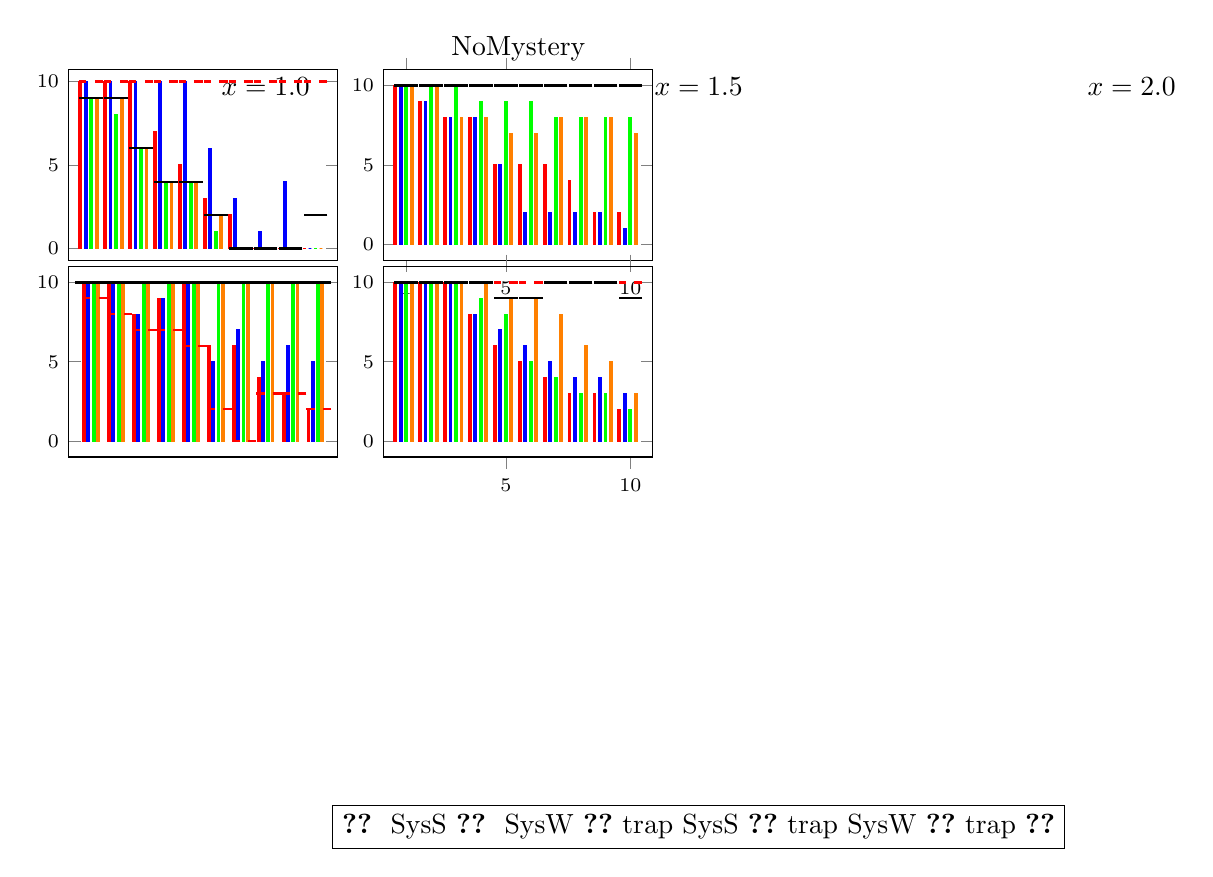
\begin{tikzpicture}
\node[] (c1) at (2.5,2.2) {$x=1.0$};
\node[] (c15) at (8,2.2) {$x=1.5$};
\node[] (c2) at (13.5,2.2) {$x=2.0$};


    \begin{axis}[
    width = 5cm,
    height=4cm,
    enlarge x limits = 0.1,
    enlarge y limits = 0.07,
    legend columns=1,
    ybar,
    bar width=1pt,
    ymin = 0,
    ymax = 10,
	compat=1.6,
	title={},
	xticklabels={,,},
	xtick style={draw=none},
	%ylabel=goals 06,
	at={(0,0)},
]
\addplot+[ybar, bar shift =-4.0pt, red,
]
plot coordinates {
(07, 2) %c_125
(08, 0) %c_125
(03, 10) %c_125
(10, 0) %c_125
(06, 3) %c_125
(09, 0) %c_125
(02, 10) %c_125
(05, 5) %c_125
(04, 7) %c_125
(01, 10) %c_125
};
\label{plot:props_hff_bu_53}
\addplot+[ybar, bar shift =-2.0pt, blue,
]
plot coordinates {
(07, 3) %c_125
(08, 1) %c_125
(03, 10) %c_125
(10, 0) %c_125
(06, 6) %c_125
(09, 4) %c_125
(02, 10) %c_125
(05, 10) %c_125
(04, 10) %c_125
(01, 10) %c_125
};
\label{plot:props_hff_td_53}
\addplot+[ybar, bar shift =0.0pt, green,
]
plot coordinates {
(07, 0) %c_125
(08, 0) %c_125
(03, 6) %c_125
(10, 0) %c_125
(06, 1) %c_125
(09, 0) %c_125
(02, 8) %c_125
(05, 4) %c_125
(04, 4) %c_125
(01, 9) %c_125
};
\label{plot:props_trap_bu_53}
\addplot+[ybar, bar shift =2.0pt, orange,
]
plot coordinates {
(07, 0) %c_125
(08, 0) %c_125
(03, 6) %c_125
(10, 0) %c_125
(06, 2) %c_125
(09, 0) %c_125
(02, 9) %c_125
(05, 4) %c_125
(04, 4) %c_125
(01, 9) %c_125
};
\label{plot:props_trap_td_53}

%lmcut
\addplot+[only marks, mark = -, mark options = {thick, red, dashed}, mark size = 0.15cm, black,
]
plot coordinates {
(02, 10)
(01, 10)
(04, 10)
(03, 10)
(07, 10)
(08, 10)
(06, 10)
(10, 10)
(05, 10)
(09, 10)
};

%trap first meta node top down
\addplot+[only marks, mark = -, mark options = {thick, black}, mark size = 0.15cm, black,
]
plot coordinates {
(01, 9)
(02, 9)
(03, 6)
(04, 4)
(05, 4)
(06, 2)
(07, 0)
(08, 0)
(09, 0)
(10, 2)
};
    \end{axis}
    \hfill
    
%\node[draw, align=center] (test) at (2,-2) {
%\ref{plot:props_hff_bu_53} props-hff-bu\\
%\ref{plot:props_hff_td_53} props-hff-td\\
%\ref{plot:props_trap_bu_53} props-trap-bu\\
%\ref{plot:props_trap_td_53} props-trap-td\\
%};



    \begin{axis}[
    width = 5cm,
    height=4cm,
    enlarge x limits = 0.1,
    enlarge y limits = 0.1,
    legend columns=1,
    ybar,
    bar width=1pt,
    ymin = 0,
    ymax = 10,
	compat=1.6,
	title=NoMystery,
	title style={yshift=-1.5ex},
	%ylabel=goals 6,
	%xticklabels={,,},
	%xtick style={draw=none},
	xtick= {1,5,10},
	at={(4cm,0)},
]
\addplot+[ybar, bar shift =-4.0pt, red,
]
plot coordinates {
(04, 8) %c_100
(09, 2) %c_100
(10, 2) %c_100
(08, 4) %c_100
(02, 9) %c_100
(07, 5) %c_100
(06, 5) %c_100
(05, 5) %c_100
(03, 8) %c_100
(01, 10) %c_100
};
\label{plot:props_bu_hff_46}
\addplot+[ybar, bar shift =-2.0pt, blue,
]
plot coordinates {
(04, 8) %c_100
(09, 2) %c_100
(10, 1) %c_100
(08, 2) %c_100
(02, 9) %c_100
(07, 2) %c_100
(06, 2) %c_100
(05, 5) %c_100
(03, 8) %c_100
(01, 10) %c_100
};
\label{plot:props_td_hff_46}
\addplot+[ybar, bar shift =0.0pt, green,
]
plot coordinates {
(04, 9) %c_100
(09, 8) %c_100
(10, 8) %c_100
(08, 8) %c_100
(02, 10) %c_100
(07, 8) %c_100
(06, 9) %c_100
(05, 9) %c_100
(03, 10) %c_100
(01, 10) %c_100
};
\label{plot:props_bu_trap_46}
\addplot+[ybar, bar shift =2.0pt, orange,
]
plot coordinates {
(04, 8) %c_100
(09, 8) %c_100
(03, 8) %c_100
(08, 8) %c_100
(02, 10) %c_100
(07, 8) %c_100
(06, 7) %c_100
(05, 7) %c_100
(10, 7) %c_100
(01, 10) %c_100
};
\label{plot:props_td_trap_46}

%lmcut
\addplot+[only marks, mark = -, mark options = {thick, red, dashed}, mark size = 0.15cm, black,
]
plot coordinates {
(01, 10)
(02, 10)
(03, 10)
(04, 10)
(05, 10)
(06, 10)
(07, 10)
(08, 10)
(09, 10)
(10, 10)
};

%trap first meta node top down
\addplot+[only marks, mark = -, mark options = {thick, black}, mark size = 0.15cm, black,
]
plot coordinates {
(01, 10)
(02, 10)
(03, 10)
(04, 10)
(05, 10)
(06, 10)
(07, 10)
(08, 10)
(09, 10)
(10, 10)
};
    \end{axis}
    \hfill
    
%\node[draw, align=center] (test) at (8,-18) {
%\ref{plot:props_bu_hff_46} props-bu-hff\\
%\ref{plot:props_td_hff_46} props-td-hff\\
%\ref{plot:props_bu_trap_46} props-bu-trap\\
%\ref{plot:props_td_trap_46} props-td-trap\\
%};



\begin{axis}[
width = 5cm,
height=4cm,
enlarge x limits = 0.1,
enlarge y limits = 0.1,
legend columns=1,
ybar,
bar width=1pt,
ymin = 0,
ymax = 10,
compat=1.6,
at={(0,-2.5cm)},
	xticklabels={,,},
	xtick style={draw=none},
]
\addplot+[ybar, bar shift =-2.5pt, red,
]
plot coordinates {
(08, 4)
(09, 3)
(01, 10)
(03, 8)
(02, 10)
(04, 9)
(05, 10)
(06, 6)
(10, 2)
(07, 6)
};
\label{plot:properties_hff_bu_52}
\addplot+[ybar, bar shift =-1.0pt, blue,
]
plot coordinates {
(01, 10)
(08, 5)
(02, 10)
(04, 9)
(03, 8)
(05, 10)
(06, 5)
(10, 5)
(07, 7)
(09, 6)
};
\label{plot:properties_hff_td_52}
\addplot+[ybar, bar shift =1.0pt, green,
]
plot coordinates {
(09, 10)
(01, 10)
(02, 10)
(04, 10)
(03, 10)
(05, 10)
(06, 10)
(10, 10)
(07, 10)
(08, 10)
};
\label{plot:properties_trap_prefop_bu_52}
\addplot+[ybar, bar shift =2.5pt, orange,
]
plot coordinates {
(01, 10)
(08, 10)
(02, 10)
(03, 10)
(04, 10)
(05, 10)
(06, 10)
(10, 10)
(07, 10)
(09, 10)
};
\label{plot:properties_trap_prefop_td_52}

%start node sysW
\addplot+[only marks, mark = -, mark options = {thick}, mark size = 0.2cm, black,
]
plot coordinates {
(02, 10)
(01, 10)
(04, 10)
(03, 10)
(07, 10)
(08, 10)
(06, 10)
(10, 10)
(05, 10)
(09, 10)
};
%optimal
\addplot+[only marks, mark = -, mark options = {thick, red, dashed}, mark size = 0.2cm, black,
]
plot coordinates {
(03, 7)
(05, 6)
(07, 0)
(09, 3)
(01, 9)
(02, 8)
(04, 7)
(06, 2)
(08, 3)
(10, 2)
};

\end{axis}


    \begin{axis}[
    width = 5cm,
    height=4cm,
    enlarge x limits = 0.1,
    enlarge y limits = 0.1,
    legend columns=1,
    ybar,
    bar width=1pt,
    ymin = 0,
    ymax = 10,
compat=1.6,
%title=c 150,
%ylabel=goals 7,
at={(4cm,-2.5cm)},
]
\addplot+[ybar, bar shift =-4.0pt, red,
]
plot coordinates {
(07, 4) %c_150
(06, 5) %c_150
(05, 6) %c_150
(09, 3) %c_150
(08, 3) %c_150
(10, 2) %c_150
(01, 10) %c_150
(04, 8) %c_150
(03, 10) %c_150
(02, 10) %c_150
};
\label{plot:props_bu_hff_49}
\addplot+[ybar, bar shift =-2.0pt, blue,
]
plot coordinates {
(07, 5) %c_150
(06, 6) %c_150
(05, 7) %c_150
(09, 4) %c_150
(08, 4) %c_150
(10, 3) %c_150
(01, 10) %c_150
(04, 8) %c_150
(03, 10) %c_150
(02, 10) %c_150
};
\label{plot:props_td_hff_49}
\addplot+[ybar, bar shift =0.0pt, green,
]
plot coordinates {
(07, 4) %c_150
(06, 5) %c_150
(05, 8) %c_150
(09, 3) %c_150
(08, 3) %c_150
(03, 10) %c_150
(01, 10) %c_150
(04, 9) %c_150
(10, 2) %c_150
(02, 10) %c_150
};
\label{plot:props_bu_trap_49}
\addplot+[ybar, bar shift =2.0pt, orange,
]
plot coordinates {
(07, 8) %c_150
(06, 9) %c_150
(05, 9) %c_150
(09, 5) %c_150
(08, 6) %c_150
(10, 3) %c_150
(01, 10) %c_150
(04, 10) %c_150
(03, 10) %c_150
(02, 10) %c_150
};
\label{plot:props_td_trap_49}

%lmcut
\addplot+[only marks, mark = -, mark options = {thick, red, dashed}, mark size = 0.15cm, black,
]
plot coordinates {
(02, 10)
(01, 10)
(04, 10)
(03, 10)
(07, 10)
(08, 10)
(06, 10)
(10, 10)
(05, 10)
(09, 10)
};

%trap first meta node top down
\addplot+[only marks, mark = -, mark options = {thick, black}, mark size = 0.15cm, black,
]
plot coordinates {
(01, 10)
(02, 10)
(03, 10)
(04, 10)
(05, 9)
(06, 9)
(07, 10)
(08, 10)
(09, 10)
(10, 9)
};
    \end{axis}
    \hfill
    
%\node[draw, align=center] (test) at (8,-18) {
%\ref{plot:props_bu_hff_49} props-bu-hff\\
%\ref{plot:props_td_hff_49} props-td-hff\\
%\ref{plot:props_bu_trap_49} props-bu-trap\\
%\ref{plot:props_td_trap_49} props-td-trap\\
%};



\node[draw] (test) at (8,-7.2) {
\ref{plot:properties_hff_bu_39} $\hff$ SysS
\ref{plot:properties_hff_td_39} $\hff$ SysW
\ref{plot:properties_trap_prefop_bu_39} trap SysS
\ref{plot:properties_trap_prefop_td_39} trap SysW
\ref{plot:baseline_sysW_node} trap
\ref{plot:baseline_lmcut} \hlmcut
};
\end{tikzpicture}

\caption{TODO}
\end{figure*}

\begin{figure*}[ht]

\tiny
\begin{tikzpicture}


\begin{axis}[
width = 7cm,
height=4cm,
enlarge x limits = 0.1,
enlarge y limits = 0.1,
ybar,
bar width=1pt,
ymin = 0,
ymax = 10,
at={(0.0\linewidth,-0.0)},
compat=1.6,
ylabel=\small \#goals 4,
]
\addplot+[ybar, bar shift =-2.5pt, red,
]
plot coordinates {
(07, 10)
(05, 10)
(04, 10)
(08, 10)
(01, 10)
(09, 10)
(03, 10)
(06, 10)
(10, 9)
(02, 10)
};
\label{plot:properties_hff_bu_39}
\addplot+[ybar, bar shift =-1.0pt, blue,
]
plot coordinates {
(07, 10)
(05, 10)
(04, 10)
(08, 10)
(09, 9)
(03, 10)
(06, 10)
(01, 10)
(10, 9)
(02, 10)
};
\label{plot:properties_hff_td_39}
\addplot+[ybar, bar shift =1.0pt, darkgreen,
]
plot coordinates {
(07, 10)
(04, 10)
(08, 10)
(09, 10)
(06, 10)
(03, 10)
(05, 10)
(01, 10)
(02, 10)
(10, 10)
};
\label{plot:properties_trap_prefop_bu_39}
\addplot+[ybar, bar shift =2.5pt, orange,
]
plot coordinates {
(07, 10)
(05, 10)
(08, 10)
(09, 10)
(06, 10)
(04, 10)
(03, 10)
(01, 10)
(02, 10)
(10, 10)
};
\label{plot:properties_trap_prefop_td_39}
\addplot+[only marks, mark = -, mark options = {thick}, mark size = 0.2cm, black,
]
plot coordinates {
(07, 10)
(05, 10)
(08, 10)
(09, 10)
(06, 10)
(04, 10)
(03, 10)
(01, 10)
(02, 10)
(10, 10)
};
\addplot+[only marks, mark = -, mark options = {thick, red, dashed}, mark size = 0.2cm, black,
]
plot coordinates {
(02, 10)
(01, 10)
(04, 10)
(03, 10)
(07, 10)
(08, 10)
(06, 10)
(10, 10)
(05, 10)
(09, 10)
};

\end{axis}
\hfill


\begin{axis}[
width = 7cm,
height=4cm,
enlarge x limits = 0.1,
enlarge y limits = 0.1,
ybar,
bar width=1pt,
ymin = 0,
ymax = 10,
at={(0.333333333333\linewidth,-0.0)},
compat=1.6,
]
\addplot+[ybar, bar shift =-2.5pt, red,
]
plot coordinates {
(05, 9)
(04, 10)
(03, 10)
(10, 1)
(02, 10)
(06, 8)
(08, 2)
(07, 5)
(09, 1)
(01, 10)
};
\label{plot:properties_hff_bu_39}
\addplot+[ybar, bar shift =-1.0pt, blue,
]
plot coordinates {
(05, 9)
(04, 10)
(03, 10)
(10, 0)
(02, 10)
(08, 2)
(07, 3)
(06, 7)
(01, 10)
(09, 0)
};
\label{plot:properties_hff_td_39}
\addplot+[ybar, bar shift =1.0pt, darkgreen,
]
plot coordinates {
(05, 8)
(04, 9)
(03, 10)
(10, 2)
(02, 10)
(08, 3)
(07, 5)
(09, 2)
(06, 6)
(01, 10)
};
\label{plot:properties_trap_prefop_bu_39}
\addplot+[ybar, bar shift =2.5pt, orange,
]
plot coordinates {
(05, 10)
(04, 10)
(03, 10)
(10, 2)
(02, 10)
(08, 4)
(07, 6)
(06, 9)
(01, 10)
(09, 3)
};
\label{plot:properties_trap_prefop_td_39}
\addplot+[only marks, mark = -, mark options = {thick}, mark size = 0.2cm, black,
]
plot coordinates {
(05, 10)
(04, 10)
(03, 10)
(10, 10)
(02, 10)
(08, 10)
(07, 10)
(06, 10)
(01, 10)
(09, 10)
};
\addplot+[only marks, mark = -, mark options = {thick, red, dashed}, mark size = 0.2cm, black,
]
plot coordinates {
(02, 10)
(01, 10)
(04, 10)
(03, 10)
(07, 10)
(08, 10)
(06, 10)
(10, 10)
(05, 10)
(09, 10)
};

\end{axis}
\hfill


\begin{axis}[
width = 7cm,
height=4cm,
enlarge x limits = 0.1,
enlarge y limits = 0.1,
ybar,
bar width=1pt,
ymin = 0,
ymax = 10,
at={(0.666666666667\linewidth,-0.0)},
compat=1.6,
]
\addplot+[ybar, bar shift =-2.5pt, red,
]
plot coordinates {
(08, 1)
(09, 0)
(01, 10)
(03, 10)
(04, 10)
(07, 2)
(02, 10)
(06, 6)
(05, 10)
(10, 0)
};
\label{plot:properties_hff_bu_39}
\addplot+[ybar, bar shift =-1.0pt, blue,
]
plot coordinates {
(08, 6)
(06, 9)
(04, 10)
(09, 5)
(01, 10)
(03, 10)
(07, 8)
(02, 10)
(05, 10)
(10, 2)
};
\label{plot:properties_hff_td_39}
\addplot+[ybar, bar shift =1.0pt, darkgreen,
]
plot coordinates {
(08, 2)
(02, 10)
(06, 5)
(04, 10)
(09, 0)
(03, 10)
(07, 3)
(01, 10)
(10, 0)
(05, 9)
};
\label{plot:properties_trap_prefop_bu_39}
\addplot+[ybar, bar shift =2.5pt, orange,
]
plot coordinates {
(08, 9)
(03, 10)
(06, 10)
(04, 10)
(09, 8)
(07, 8)
(02, 10)
(01, 10)
(10, 5)
(05, 10)
};
\label{plot:properties_trap_prefop_td_39}
\addplot+[only marks, mark = -, mark options = {thick}, mark size = 0.2cm, black,
]
plot coordinates {
(08, 9)
(03, 10)
(06, 10)
(04, 10)
(09, 8)
(07, 9)
(02, 10)
(01, 10)
(10, 7)
(05, 10)
};
\addplot+[only marks, mark = -, mark options = {thick, red, dashed}, mark size = 0.2cm, black,
]
plot coordinates {
(02, 10)
(01, 10)
(04, 10)
(03, 10)
(07, 10)
(08, 10)
(06, 10)
(10, 10)
(05, 10)
(09, 10)
};

\end{axis}
\hfill


\begin{axis}[
width = 7cm,
height=4cm,
enlarge x limits = 0.1,
enlarge y limits = 0.1,
ybar,
bar width=1pt,
ymin = 0,
ymax = 10,
at={(0.0\linewidth,-160.0)},
compat=1.6,
ylabel=\small \#goals 5,
]
\addplot+[ybar, bar shift =-2.5pt, red,
]
plot coordinates {
(01, 10)
(08, 9)
(03, 10)
(02, 10)
(09, 9)
(05, 10)
(04, 10)
(07, 9)
(06, 10)
(10, 9)
};
\label{plot:properties_hff_bu_39}
\addplot+[ybar, bar shift =-1.0pt, blue,
]
plot coordinates {
(01, 10)
(08, 6)
(03, 10)
(02, 10)
(09, 5)
(05, 10)
(04, 10)
(07, 7)
(06, 9)
(10, 2)
};
\label{plot:properties_hff_td_39}
\addplot+[ybar, bar shift =1.0pt, darkgreen,
]
plot coordinates {
(01, 10)
(08, 10)
(03, 10)
(02, 10)
(09, 10)
(05, 10)
(04, 10)
(07, 10)
(06, 10)
(10, 10)
};
\label{plot:properties_trap_prefop_bu_39}
\addplot+[ybar, bar shift =2.5pt, orange,
]
plot coordinates {
(01, 10)
(08, 10)
(03, 10)
(02, 10)
(09, 10)
(05, 10)
(04, 10)
(07, 10)
(06, 10)
(10, 10)
};
\label{plot:properties_trap_prefop_td_39}
\addplot+[only marks, mark = -, mark options = {thick}, mark size = 0.2cm, black,
]
plot coordinates {
(01, 10)
(08, 10)
(03, 10)
(02, 10)
(09, 10)
(05, 10)
(04, 10)
(07, 10)
(06, 10)
(10, 10)
};
\addplot+[only marks, mark = -, mark options = {thick, red, dashed}, mark size = 0.2cm, black,
]
plot coordinates {
(02, 10)
(01, 10)
(04, 10)
(03, 10)
(07, 10)
(08, 10)
(06, 10)
(10, 10)
(05, 10)
(09, 10)
};

\end{axis}
\hfill


\begin{axis}[
width = 7cm,
height=4cm,
enlarge x limits = 0.1,
enlarge y limits = 0.1,
ybar,
bar width=1pt,
ymin = 0,
ymax = 10,
at={(0.333333333333\linewidth,-160.0)},
compat=1.6,
]
\addplot+[ybar, bar shift =-2.5pt, red,
]
plot coordinates {
(05, 5)
(06, 2)
(10, 0)
(03, 10)
(04, 9)
(01, 10)
(09, 0)
(02, 10)
(07, 1)
(08, 1)
};
\label{plot:properties_hff_bu_39}
\addplot+[ybar, bar shift =-1.0pt, blue,
]
plot coordinates {
(05, 7)
(06, 4)
(10, 1)
(03, 10)
(04, 9)
(01, 10)
(09, 1)
(02, 10)
(07, 1)
(08, 1)
};
\label{plot:properties_hff_td_39}
\addplot+[ybar, bar shift =1.0pt, darkgreen,
]
plot coordinates {
(05, 6)
(06, 2)
(10, 1)
(03, 10)
(04, 10)
(01, 10)
(09, 1)
(02, 10)
(07, 1)
(08, 1)
};
\label{plot:properties_trap_prefop_bu_39}
\addplot+[ybar, bar shift =2.5pt, orange,
]
plot coordinates {
(05, 9)
(06, 6)
(10, 2)
(03, 10)
(04, 10)
(01, 10)
(09, 2)
(02, 10)
(07, 4)
(08, 3)
};
\label{plot:properties_trap_prefop_td_39}
\addplot+[only marks, mark = -, mark options = {thick}, mark size = 0.2cm, black,
]
plot coordinates {
(05, 10)
(06, 9)
(10, 9)
(03, 10)
(04, 10)
(01, 10)
(09, 9)
(02, 10)
(07, 9)
(08, 9)
};
\addplot+[only marks, mark = -, mark options = {thick, red, dashed}, mark size = 0.2cm, black,
]
plot coordinates {
(02, 10)
(01, 10)
(04, 10)
(03, 10)
(07, 10)
(08, 10)
(06, 10)
(10, 10)
(05, 10)
(09, 10)
};

\end{axis}
\hfill


\begin{axis}[
width = 7cm,
height=4cm,
enlarge x limits = 0.1,
enlarge y limits = 0.1,
ybar,
bar width=1pt,
ymin = 0,
ymax = 10,
at={(0.666666666667\linewidth,-160.0)},
compat=1.6,
]
\addplot+[ybar, bar shift =-2.5pt, red,
]
plot coordinates {
(03, 10)
(04, 7)
(05, 3)
(09, 0)
(01, 10)
(02, 10)
(08, 0)
(06, 1)
(10, 0)
(07, 0)
};
\label{plot:properties_hff_bu_39}
\addplot+[ybar, bar shift =-1.0pt, blue,
]
plot coordinates {
(03, 10)
(04, 8)
(05, 7)
(09, 5)
(01, 10)
(02, 10)
(08, 5)
(06, 7)
(10, 4)
(07, 6)
};
\label{plot:properties_hff_td_39}
\addplot+[ybar, bar shift =1.0pt, darkgreen,
]
plot coordinates {
(03, 9)
(04, 6)
(05, 1)
(09, 0)
(01, 10)
(02, 10)
(08, 0)
(06, 1)
(10, 0)
(07, 0)
};
\label{plot:properties_trap_prefop_bu_39}
\addplot+[ybar, bar shift =2.5pt, orange,
]
plot coordinates {
(03, 10)
(04, 10)
(05, 8)
(09, 5)
(01, 10)
(02, 10)
(08, 6)
(06, 7)
(10, 4)
(07, 8)
};
\label{plot:properties_trap_prefop_td_39}
\addplot+[only marks, mark = -, mark options = {thick}, mark size = 0.2cm, black,
]
plot coordinates {
(03, 10)
(04, 10)
(05, 9)
(09, 8)
(01, 10)
(02, 10)
(08, 8)
(06, 8)
(10, 8)
(07, 8)
};
\addplot+[only marks, mark = -, mark options = {thick, red, dashed}, mark size = 0.2cm, black,
]
plot coordinates {
(02, 10)
(01, 10)
(04, 10)
(03, 10)
(07, 10)
(08, 10)
(06, 10)
(10, 10)
(05, 10)
(09, 10)
};

\end{axis}
\hfill


\begin{axis}[
width = 7cm,
height=4cm,
enlarge x limits = 0.1,
enlarge y limits = 0.1,
ybar,
bar width=1pt,
ymin = 0,
ymax = 10,
at={(0.0\linewidth,-320.0)},
compat=1.6,
ylabel=\small \#goals 6,
]
\addplot+[ybar, bar shift =-2.5pt, red,
]
plot coordinates {
(08, 2)
(09, 2)
(01, 10)
(10, 2)
(06, 5)
(07, 4)
(04, 8)
(05, 5)
(02, 9)
(03, 8)
};
\label{plot:properties_hff_bu_39}
\addplot+[ybar, bar shift =-1.0pt, blue,
]
plot coordinates {
(08, 2)
(09, 2)
(01, 10)
(10, 2)
(06, 2)
(07, 2)
(04, 7)
(05, 4)
(02, 9)
(03, 8)
};
\label{plot:properties_hff_td_39}
\addplot+[ybar, bar shift =1.0pt, darkgreen,
]
plot coordinates {
(08, 8)
(09, 8)
(01, 10)
(10, 8)
(06, 9)
(07, 8)
(04, 10)
(05, 9)
(02, 10)
(03, 10)
};
\label{plot:properties_trap_prefop_bu_39}
\addplot+[ybar, bar shift =2.5pt, orange,
]
plot coordinates {
(08, 8)
(09, 8)
(01, 10)
(10, 7)
(06, 7)
(07, 8)
(04, 8)
(05, 7)
(02, 10)
(03, 8)
};
\label{plot:properties_trap_prefop_td_39}
\addplot+[only marks, mark = -, mark options = {thick}, mark size = 0.2cm, black,
]
plot coordinates {
(08, 10)
(09, 10)
(01, 10)
(10, 10)
(06, 10)
(07, 10)
(04, 10)
(05, 10)
(02, 10)
(03, 10)
};
\addplot+[only marks, mark = -, mark options = {thick, red, dashed}, mark size = 0.2cm, black,
]
plot coordinates {
(02, 10)
(01, 10)
(04, 10)
(03, 10)
(07, 10)
(08, 10)
(06, 10)
(10, 10)
(05, 10)
(09, 10)
};

\end{axis}
\hfill


\begin{axis}[
width = 7cm,
height=4cm,
enlarge x limits = 0.1,
enlarge y limits = 0.1,
ybar,
bar width=1pt,
ymin = 0,
ymax = 10,
at={(0.333333333333\linewidth,-320.0)},
compat=1.6,
]
\addplot+[ybar, bar shift =-2.5pt, red,
]
plot coordinates {
(06, 1)
(10, 0)
(05, 3)
(08, 1)
(07, 1)
(02, 10)
(09, 0)
(01, 10)
(04, 7)
(03, 9)
};
\label{plot:properties_hff_bu_39}
\addplot+[ybar, bar shift =-1.0pt, blue,
]
plot coordinates {
(06, 2)
(10, 0)
(05, 4)
(08, 0)
(07, 0)
(02, 10)
(09, 0)
(01, 10)
(04, 7)
(03, 10)
};
\label{plot:properties_hff_td_39}
\addplot+[ybar, bar shift =1.0pt, darkgreen,
]
plot coordinates {
(06, 2)
(10, 2)
(05, 2)
(08, 2)
(07, 2)
(02, 10)
(09, 2)
(01, 10)
(04, 4)
(03, 7)
};
\label{plot:properties_trap_prefop_bu_39}
\addplot+[ybar, bar shift =2.5pt, orange,
]
plot coordinates {
(06, 3)
(10, 3)
(05, 4)
(08, 3)
(07, 3)
(02, 10)
(09, 3)
(01, 10)
(04, 6)
(03, 8)
};
\label{plot:properties_trap_prefop_td_39}
\addplot+[only marks, mark = -, mark options = {thick}, mark size = 0.2cm, black,
]
plot coordinates {
(06, 7)
(10, 7)
(05, 7)
(08, 7)
(07, 7)
(02, 10)
(09, 5)
(01, 10)
(04, 7)
(03, 8)
};
\addplot+[only marks, mark = -, mark options = {thick, red, dashed}, mark size = 0.2cm, black,
]
plot coordinates {
(02, 10)
(01, 10)
(04, 10)
(03, 10)
(07, 10)
(08, 10)
(06, 10)
(10, 10)
(05, 10)
(09, 10)
};

\end{axis}
\hfill


\begin{axis}[
width = 7cm,
height=4cm,
enlarge x limits = 0.1,
enlarge y limits = 0.1,
ybar,
bar width=1pt,
ymin = 0,
ymax = 10,
at={(0.666666666667\linewidth,-320.0)},
compat=1.6,
]
\addplot+[ybar, bar shift =-2.5pt, red,
]
plot coordinates {
(02, 8)
(01, 10)
(04, 3)
(03, 4)
(06, 1)
(10, 0)
(05, 3)
(09, 0)
(08, 0)
(07, 0)
};
\label{plot:properties_hff_bu_39}
\addplot+[ybar, bar shift =-1.0pt, blue,
]
plot coordinates {
(02, 9)
(01, 10)
(04, 6)
(03, 7)
(07, 4)
(08, 3)
(06, 4)
(10, 1)
(05, 6)
(09, 1)
};
\label{plot:properties_hff_td_39}
\addplot+[ybar, bar shift =1.0pt, darkgreen,
]
plot coordinates {
(02, 10)
(01, 10)
(04, 4)
(03, 5)
(08, 0)
(06, 1)
(10, 0)
(05, 2)
(09, 0)
(07, 0)
};
\label{plot:properties_trap_prefop_bu_39}
\addplot+[ybar, bar shift =2.5pt, orange,
]
plot coordinates {
(02, 10)
(01, 10)
(04, 7)
(03, 8)
(07, 5)
(08, 4)
(06, 7)
(10, 3)
(05, 7)
(09, 3)
};
\label{plot:properties_trap_prefop_td_39}
\addplot+[only marks, mark = -, mark options = {thick}, mark size = 0.2cm, black,
]
plot coordinates {
(02, 10)
(01, 10)
(04, 7)
(03, 8)
(07, 7)
(08, 6)
(06, 7)
(10, 5)
(05, 7)
(09, 5)
};
\label{plot:baseline_sysW_node}
\addplot+[only marks, mark = -, mark options = {thick, red, dashed}, mark size = 0.2cm, black,
]
plot coordinates {
(02, 10)
(01, 10)
(04, 10)
(03, 10)
(07, 10)
(08, 10)
(06, 10)
(10, 10)
(05, 10)
(09, 10)
};
\label{plot:baseline_lmcut}

\end{axis}
\hfill

\node[] (c1) at (2.5,2.8) {\small $x=1.0$};
\node[] (c15) at (8.4,2.8) {\small $x=1.5$};
\node[] (c2) at (14.3,2.8) {\small $x=2.0$};

\node[draw] (test) at (8,-7.5) {
\ref{plot:properties_hff_bu_39}  SysS
\ref{plot:properties_hff_td_39}  SysW
\ref{plot:properties_trap_prefop_bu_39} SysS trap 
\ref{plot:properties_trap_prefop_td_39} SysW trap 
\ref{plot:baseline_lmcut} \hlmcut
\ref{plot:baseline_sysW_node} trap
};

\end{tikzpicture}
\hfill

\caption{nomystery: reference coverage first node in top-down meta search tree;
	optimal coverage always 10}
\end{figure*}

\begin{figure*}[ht]

\tiny
\begin{tikzpicture}


\begin{axis}[
width = 7cm,
height=4cm,
enlarge x limits = 0.1,
enlarge y limits = 0.1,
ybar,
bar width=1pt,
ymin = 0,
ymax = 10,
at={(0.0\linewidth,-0.0)},
compat=1.6,
title=c 100,
ylabel=goals 4,
]
\addplot+[ybar, bar shift =-2.5pt, red,
]
plot coordinates {
(04, 10)
(03, 10)
(02, 10)
(09, 10)
(01, 10)
(08, 10)
(07, 10)
(10, 10)
(06, 10)
(05, 10)
};
\label{plot:properties_hff_bu_47}
\addplot+[ybar, bar shift =-1.0pt, blue,
]
plot coordinates {
(04, 10)
(03, 10)
(02, 10)
(09, 10)
(01, 10)
(08, 10)
(07, 10)
(10, 10)
(06, 10)
(05, 10)
};
\label{plot:properties_hff_td_47}
\addplot+[ybar, bar shift =1.0pt, darkgreen,
]
plot coordinates {
(04, 10)
(03, 10)
(02, 10)
(09, 10)
(01, 10)
(08, 10)
(07, 10)
(10, 10)
(06, 10)
(05, 10)
};
\label{plot:properties_trap_prefop_bu_47}
\addplot+[ybar, bar shift =2.5pt, orange,
]
plot coordinates {
(04, 10)
(03, 10)
(02, 10)
(09, 10)
(01, 10)
(08, 10)
(07, 10)
(10, 10)
(06, 10)
(05, 10)
};
\label{plot:properties_trap_prefop_td_47}
\addplot+[only marks, mark = -, mark options = {thick}, mark size = 0.2cm, black,
]
plot coordinates {
(04, 10)
(03, 10)
(02, 10)
(09, 10)
(01, 10)
(08, 10)
(07, 10)
(10, 10)
(06, 10)
(05, 10)
};

\end{axis}
\hfill


\begin{axis}[
width = 7cm,
height=4cm,
enlarge x limits = 0.1,
enlarge y limits = 0.1,
ybar,
bar width=1pt,
ymin = 0,
ymax = 10,
at={(0.333333333333\linewidth,-0.0)},
compat=1.6,
title=c 150,
]
\addplot+[ybar, bar shift =-2.5pt, red,
]
plot coordinates {
(07, 10)
(08, 10)
(09, 10)
(01, 10)
(02, 10)
(03, 10)
(04, 10)
(05, 10)
(06, 10)
(10, 10)
};
\label{plot:properties_hff_bu_47}
\addplot+[ybar, bar shift =-1.0pt, blue,
]
plot coordinates {
(07, 10)
(08, 10)
(09, 8)
(01, 10)
(02, 10)
(03, 10)
(04, 10)
(05, 10)
(06, 10)
(10, 4)
};
\label{plot:properties_hff_td_47}
\addplot+[ybar, bar shift =1.0pt, darkgreen,
]
plot coordinates {
(07, 10)
(08, 9)
(09, 9)
(01, 10)
(02, 10)
(03, 10)
(04, 10)
(05, 10)
(06, 10)
(10, 9)
};
\label{plot:properties_trap_prefop_bu_47}
\addplot+[ybar, bar shift =2.5pt, orange,
]
plot coordinates {
(07, 10)
(08, 10)
(09, 10)
(01, 10)
(02, 10)
(03, 10)
(04, 10)
(05, 10)
(06, 10)
(10, 10)
};
\label{plot:properties_trap_prefop_td_47}
\addplot+[only marks, mark = -, mark options = {thick}, mark size = 0.2cm, black,
]
plot coordinates {
(07, 10)
(08, 10)
(09, 10)
(01, 10)
(02, 10)
(03, 10)
(04, 10)
(05, 10)
(06, 10)
(10, 10)
};

\end{axis}
\hfill


\begin{axis}[
width = 7cm,
height=4cm,
enlarge x limits = 0.1,
enlarge y limits = 0.1,
ybar,
bar width=1pt,
ymin = 0,
ymax = 10,
at={(0.666666666667\linewidth,-0.0)},
compat=1.6,
title=c 200,
]
\addplot+[ybar, bar shift =-2.5pt, red,
]
plot coordinates {
(08, 10)
(03, 10)
(04, 10)
(05, 10)
(06, 10)
(10, 9)
(07, 10)
(01, 10)
(09, 10)
(02, 10)
};
\label{plot:properties_hff_bu_47}
\addplot+[ybar, bar shift =-1.0pt, blue,
]
plot coordinates {
(05, 10)
(04, 10)
(02, 10)
(10, 8)
(07, 10)
(03, 10)
(08, 10)
(01, 10)
(09, 8)
(06, 10)
};
\label{plot:properties_hff_td_47}
\addplot+[ybar, bar shift =1.0pt, darkgreen,
]
plot coordinates {
(08, 10)
(03, 10)
(05, 10)
(04, 10)
(02, 10)
(06, 10)
(10, 8)
(07, 10)
(01, 10)
(09, 9)
};
\label{plot:properties_trap_prefop_bu_47}
\addplot+[ybar, bar shift =2.5pt, orange,
]
plot coordinates {
(03, 10)
(05, 10)
(04, 10)
(10, 10)
(07, 10)
(08, 10)
(01, 10)
(09, 10)
(06, 10)
(02, 10)
};
\label{plot:properties_trap_prefop_td_47}
\addplot+[only marks, mark = -, mark options = {thick}, mark size = 0.2cm, black,
]
plot coordinates {
(03, 10)
(05, 10)
(04, 10)
(10, 10)
(07, 10)
(08, 10)
(01, 10)
(09, 10)
(06, 10)
(02, 10)
};

\end{axis}
\hfill


\begin{axis}[
width = 7cm,
height=4cm,
enlarge x limits = 0.1,
enlarge y limits = 0.1,
ybar,
bar width=1pt,
ymin = 0,
ymax = 10,
at={(0.0\linewidth,-160.0)},
compat=1.6,
ylabel=goals 5,
]
\addplot+[ybar, bar shift =-2.5pt, red,
]
plot coordinates {
(03, 10)
(08, 10)
(09, 10)
(01, 10)
(06, 10)
(07, 10)
(04, 10)
(05, 10)
(10, 10)
(02, 10)
};
\label{plot:properties_hff_bu_47}
\addplot+[ybar, bar shift =-1.0pt, blue,
]
plot coordinates {
(03, 10)
(08, 9)
(09, 7)
(01, 10)
(06, 10)
(07, 10)
(04, 10)
(05, 10)
(10, 4)
(02, 10)
};
\label{plot:properties_hff_td_47}
\addplot+[ybar, bar shift =1.0pt, darkgreen,
]
plot coordinates {
(03, 10)
(08, 10)
(09, 10)
(01, 10)
(06, 10)
(07, 10)
(04, 10)
(05, 10)
(10, 10)
(02, 10)
};
\label{plot:properties_trap_prefop_bu_47}
\addplot+[ybar, bar shift =2.5pt, orange,
]
plot coordinates {
(03, 10)
(08, 10)
(09, 10)
(01, 10)
(06, 10)
(07, 10)
(04, 10)
(05, 10)
(10, 10)
(02, 10)
};
\label{plot:properties_trap_prefop_td_47}
\addplot+[only marks, mark = -, mark options = {thick}, mark size = 0.2cm, black,
]
plot coordinates {
(03, 10)
(08, 10)
(09, 10)
(01, 10)
(06, 10)
(07, 10)
(04, 10)
(05, 10)
(10, 10)
(02, 10)
};

\end{axis}
\hfill


\begin{axis}[
width = 7cm,
height=4cm,
enlarge x limits = 0.1,
enlarge y limits = 0.1,
ybar,
bar width=1pt,
ymin = 0,
ymax = 10,
at={(0.333333333333\linewidth,-160.0)},
compat=1.6,
]
\addplot+[ybar, bar shift =-2.5pt, red,
]
plot coordinates {
(02, 10)
(10, 3)
(05, 10)
(04, 10)
(07, 7)
(06, 9)
(09, 3)
(01, 10)
(08, 6)
(03, 10)
};
\label{plot:properties_hff_bu_47}
\addplot+[ybar, bar shift =-1.0pt, blue,
]
plot coordinates {
(02, 10)
(10, 2)
(04, 10)
(05, 10)
(07, 7)
(06, 9)
(09, 2)
(01, 10)
(08, 5)
(03, 10)
};
\label{plot:properties_hff_td_47}
\addplot+[ybar, bar shift =1.0pt, darkgreen,
]
plot coordinates {
(02, 10)
(10, 5)
(04, 10)
(05, 10)
(07, 9)
(06, 10)
(09, 8)
(01, 10)
(08, 8)
(03, 10)
};
\label{plot:properties_trap_prefop_bu_47}
\addplot+[ybar, bar shift =2.5pt, orange,
]
plot coordinates {
(02, 10)
(10, 7)
(05, 10)
(04, 10)
(07, 10)
(06, 10)
(09, 10)
(01, 10)
(08, 10)
(03, 10)
};
\label{plot:properties_trap_prefop_td_47}
\addplot+[only marks, mark = -, mark options = {thick}, mark size = 0.2cm, black,
]
plot coordinates {
(02, 10)
(10, 10)
(05, 10)
(04, 10)
(07, 10)
(06, 10)
(09, 10)
(01, 10)
(08, 10)
(03, 10)
};

\end{axis}
\hfill


\begin{axis}[
width = 7cm,
height=4cm,
enlarge x limits = 0.1,
enlarge y limits = 0.1,
ybar,
bar width=1pt,
ymin = 0,
ymax = 10,
at={(0.666666666667\linewidth,-160.0)},
compat=1.6,
]
\addplot+[ybar, bar shift =-2.5pt, red,
]
plot coordinates {
(03, 10)
(02, 10)
(10, 8)
(05, 10)
(04, 10)
(07, 9)
(06, 10)
(09, 9)
(01, 10)
(08, 9)
};
\label{plot:properties_hff_bu_47}
\addplot+[ybar, bar shift =-1.0pt, blue,
]
plot coordinates {
(03, 10)
(02, 10)
(10, 8)
(05, 10)
(04, 10)
(07, 9)
(06, 10)
(09, 9)
(01, 10)
(08, 9)
};
\label{plot:properties_hff_td_47}
\addplot+[ybar, bar shift =1.0pt, darkgreen,
]
plot coordinates {
(03, 10)
(02, 10)
(10, 6)
(05, 10)
(04, 10)
(07, 9)
(06, 10)
(09, 7)
(01, 10)
(08, 8)
};
\label{plot:properties_trap_prefop_bu_47}
\addplot+[ybar, bar shift =2.5pt, orange,
]
plot coordinates {
(03, 10)
(02, 10)
(10, 9)
(05, 10)
(04, 10)
(07, 10)
(06, 10)
(09, 10)
(01, 10)
(08, 10)
};
\label{plot:properties_trap_prefop_td_47}
\addplot+[only marks, mark = -, mark options = {thick}, mark size = 0.2cm, black,
]
plot coordinates {
(03, 10)
(02, 10)
(10, 10)
(05, 10)
(04, 10)
(07, 10)
(06, 10)
(09, 10)
(01, 10)
(08, 10)
};

\end{axis}
\hfill


\begin{axis}[
width = 7cm,
height=4cm,
enlarge x limits = 0.1,
enlarge y limits = 0.1,
ybar,
bar width=1pt,
ymin = 0,
ymax = 10,
at={(0.0\linewidth,-320.0)},
compat=1.6,
ylabel=goals 6,
]
\addplot+[ybar, bar shift =-2.5pt, red,
]
plot coordinates {
(10, 7)
(03, 10)
(05, 10)
(06, 10)
(01, 10)
(02, 10)
(09, 8)
(08, 9)
(07, 9)
(04, 10)
};
\label{plot:properties_hff_bu_47}
\addplot+[ybar, bar shift =-1.0pt, blue,
]
plot coordinates {
(10, 0)
(09, 0)
(02, 10)
(04, 10)
(05, 9)
(07, 4)
(06, 8)
(01, 10)
(08, 1)
(03, 10)
};
\label{plot:properties_hff_td_47}
\addplot+[ybar, bar shift =1.0pt, darkgreen,
]
plot coordinates {
(10, 10)
(04, 10)
(05, 10)
(06, 10)
(01, 10)
(02, 10)
(09, 10)
(08, 10)
(07, 10)
(03, 10)
};
\label{plot:properties_trap_prefop_bu_47}
\addplot+[ybar, bar shift =2.5pt, orange,
]
plot coordinates {
(10, 10)
(09, 10)
(03, 10)
(04, 10)
(05, 10)
(07, 10)
(06, 10)
(01, 10)
(02, 10)
(08, 10)
};
\label{plot:properties_trap_prefop_td_47}
\addplot+[only marks, mark = -, mark options = {thick}, mark size = 0.2cm, black,
]
plot coordinates {
(10, 10)
(09, 10)
(03, 10)
(04, 10)
(05, 10)
(07, 10)
(06, 10)
(01, 10)
(02, 10)
(08, 10)
};

\end{axis}
\hfill


\begin{axis}[
width = 7cm,
height=4cm,
enlarge x limits = 0.1,
enlarge y limits = 0.1,
ybar,
bar width=1pt,
ymin = 0,
ymax = 10,
at={(0.333333333333\linewidth,-320.0)},
compat=1.6,
]
\addplot+[ybar, bar shift =-2.5pt, red,
]
plot coordinates {
(10, 2)
(02, 10)
(03, 10)
(08, 3)
(01, 10)
(09, 2)
(06, 5)
(07, 3)
(04, 9)
(05, 8)
};
\label{plot:properties_hff_bu_47}
\addplot+[ybar, bar shift =-1.0pt, blue,
]
plot coordinates {
(10, 3)
(02, 10)
(03, 10)
(08, 3)
(01, 10)
(09, 3)
(06, 5)
(07, 3)
(04, 9)
(05, 8)
};
\label{plot:properties_hff_td_47}
\addplot+[ybar, bar shift =1.0pt, darkgreen,
]
plot coordinates {
(10, 4)
(02, 10)
(03, 10)
(08, 6)
(01, 10)
(09, 5)
(06, 10)
(07, 7)
(04, 10)
(05, 10)
};
\label{plot:properties_trap_prefop_bu_47}
\addplot+[ybar, bar shift =2.5pt, orange,
]
plot coordinates {
(10, 5)
(02, 10)
(03, 10)
(08, 8)
(01, 10)
(09, 6)
(06, 10)
(07, 9)
(04, 10)
(05, 10)
};
\label{plot:properties_trap_prefop_td_47}
\addplot+[only marks, mark = -, mark options = {thick}, mark size = 0.2cm, black,
]
plot coordinates {
(10, 10)
(02, 10)
(03, 10)
(08, 10)
(01, 10)
(09, 10)
(06, 10)
(07, 10)
(04, 10)
(05, 10)
};

\end{axis}
\hfill


\begin{axis}[
width = 7cm,
height=4cm,
enlarge x limits = 0.1,
enlarge y limits = 0.1,
ybar,
bar width=1pt,
ymin = 0,
ymax = 10,
at={(0.666666666667\linewidth,-320.0)},
compat=1.6,
]
\addplot+[ybar, bar shift =-2.5pt, red,
]
plot coordinates {
(04, 10)
(05, 10)
(02, 10)
(03, 10)
(08, 8)
(09, 8)
(01, 10)
(06, 9)
(07, 8)
(10, 7)
};
\label{plot:properties_hff_bu_47}
\addplot+[ybar, bar shift =-1.0pt, blue,
]
plot coordinates {
(04, 10)
(05, 10)
(02, 10)
(03, 10)
(08, 8)
(09, 8)
(01, 10)
(06, 9)
(07, 9)
(10, 7)
};
\label{plot:properties_hff_td_47}
\addplot+[ybar, bar shift =1.0pt, darkgreen,
]
plot coordinates {
(04, 10)
(05, 10)
(02, 10)
(03, 10)
(08, 6)
(09, 4)
(01, 10)
(06, 10)
(07, 7)
(10, 3)
};
\label{plot:properties_trap_prefop_bu_47}
\addplot+[ybar, bar shift =2.5pt, orange,
]
plot coordinates {
(04, 10)
(05, 10)
(02, 10)
(03, 10)
(08, 10)
(09, 9)
(01, 10)
(06, 10)
(07, 10)
(10, 8)
};
\label{plot:properties_trap_prefop_td_47}
\addplot+[only marks, mark = -, mark options = {thick}, mark size = 0.2cm, black,
]
plot coordinates {
(04, 10)
(05, 10)
(02, 10)
(03, 10)
(08, 10)
(09, 10)
(01, 10)
(06, 10)
(07, 10)
(10, 10)
};

\end{axis}
\hfill

\node[draw] (test) at (8,-8) {
\ref{plot:properties_hff_bu_47} properties-hff-bu
\ref{plot:properties_hff_td_47} properties-hff-td
\ref{plot:properties_trap_prefop_bu_47} properties-trap-prefop-bu
\ref{plot:properties_trap_prefop_td_47} properties-trap-prefop-td
};

\end{tikzpicture}
\hfill

\caption{TPP: reference coverage first node in top-down meta search tree;
	optimal coverage always 10}
\end{figure*}

\begin{figure*}[ht]

\tiny
\begin{tikzpicture}


\begin{axis}[
width = 7cm,
height=4cm,
enlarge x limits = 0.1,
enlarge y limits = 0.1,
ybar,
bar width=1pt,
ymin = 0,
ymax = 10,
at={(0.0\linewidth,-0.0)},
compat=1.6,
title=c 100,
ylabel=goals 05,
]
\addplot+[ybar, bar shift =-2.5pt, red,
]
plot coordinates {
(05, 10)
(04, 10)
(06, 9)
(02, 10)
(10, 6)
(01, 10)
(08, 9)
(09, 7)
(03, 10)
(07, 8)
};
\label{plot:properties_hff_bu_38}
\addplot+[ybar, bar shift =-0.5pt, blue,
]
plot coordinates {
(06, 9)
(10, 4)
(05, 10)
(04, 10)
(02, 10)
(01, 10)
(08, 5)
(09, 5)
(07, 7)
(03, 10)
};
\label{plot:properties_hff_td_38}
\addplot+[ybar, bar shift =0.5pt, darkgreen,
]
plot coordinates {
(06, 10)
(10, 10)
(05, 10)
(04, 10)
(03, 10)
(02, 10)
(01, 10)
(08, 10)
(09, 10)
(07, 10)
};
\label{plot:properties_trap_prefop_bu_38}
\addplot+[ybar, bar shift =2.5pt, orange,
]
plot coordinates {
(06, 10)
(05, 10)
(03, 10)
(07, 10)
(10, 10)
(02, 10)
(01, 10)
(08, 10)
(09, 10)
(04, 10)
};
\label{plot:properties_trap_prefop_td_38}

\addplot+[only marks, mark=-, mark options={thick}, mark size=0.2cm, black]
plot coordinates {
(1, 10)
(2, 10)
(3, 9)
(4, 8)
(5, 8)
(6, 6)
(7, 4)
(8, 6)
(9, 6)
(10, 4)
};
\end{axis}
\hfill


\begin{axis}[
width = 7cm,
height=4cm,
enlarge x limits = 0.1,
enlarge y limits = 0.1,
ybar,
bar width=1pt,
ymin = 0,
ymax = 10,
at={(0.333333333333\linewidth,-0.0)},
compat=1.6,
title=c 150,
]
\addplot+[ybar, bar shift =-2.5pt, red,
]
plot coordinates {
(08, 5)
(01, 10)
(09, 5)
(06, 8)
(07, 5)
(04, 9)
(05, 10)
(10, 4)
(02, 10)
(03, 9)
};
\label{plot:properties_hff_bu_38}
\addplot+[ybar, bar shift =-0.5pt, blue,
]
plot coordinates {
(01, 10)
(08, 4)
(09, 4)
(06, 4)
(07, 4)
(04, 9)
(05, 9)
(10, 4)
(02, 10)
(03, 9)
};
\label{plot:properties_hff_td_38}
\addplot+[ybar, bar shift =0.5pt, darkgreen,
]
plot coordinates {
(08, 10)
(01, 10)
(09, 10)
(06, 10)
(07, 10)
(04, 10)
(05, 10)
(10, 10)
(02, 10)
(03, 10)
};
\label{plot:properties_trap_prefop_bu_38}
\addplot+[ybar, bar shift =2.5pt, orange,
]
plot coordinates {
(08, 10)
(01, 10)
(09, 10)
(06, 10)
(07, 10)
(04, 10)
(05, 10)
(10, 10)
(02, 10)
(03, 10)
};
\label{plot:properties_trap_prefop_td_38}

\end{axis}
\hfill


\begin{axis}[
width = 7cm,
height=4cm,
enlarge x limits = 0.1,
enlarge y limits = 0.1,
ybar,
bar width=1pt,
ymin = 0,
ymax = 10,
at={(0.666666666667\linewidth,-0.0)},
compat=1.6,
title=c 200,
]
\addplot+[ybar, bar shift =-2.5pt, red,
]
plot coordinates {
(08, 8)
(04, 10)
(05, 10)
(10, 6)
(02, 10)
(03, 10)
(09, 9)
(01, 10)
(06, 7)
(07, 6)
};
\label{plot:properties_hff_bu_38}
\addplot+[ybar, bar shift =-0.5pt, blue,
]
plot coordinates {
(04, 10)
(05, 10)
(10, 7)
(02, 10)
(03, 10)
(08, 8)
(09, 9)
(01, 10)
(06, 7)
(07, 6)
};
\label{plot:properties_hff_td_38}
\addplot+[ybar, bar shift =0.5pt, darkgreen,
]
plot coordinates {
(04, 10)
(05, 10)
(10, 10)
(02, 10)
(03, 10)
(08, 10)
(09, 10)
(01, 10)
(06, 10)
(07, 10)
};
\label{plot:properties_trap_prefop_bu_38}
\addplot+[ybar, bar shift =2.5pt, orange,
]
plot coordinates {
(04, 10)
(05, 10)
(10, 10)
(02, 10)
(03, 10)
(08, 10)
(09, 10)
(01, 10)
(06, 10)
(07, 10)
};
\label{plot:properties_trap_prefop_td_38}

\end{axis}
\hfill


\begin{axis}[
width = 7cm,
height=4cm,
enlarge x limits = 0.1,
enlarge y limits = 0.1,
ybar,
bar width=1pt,
ymin = 0,
ymax = 10,
at={(0.0\linewidth,-160.0)},
compat=1.6,
ylabel=goals 06,
]
\addplot+[ybar, bar shift =-2.5pt, red,
]
plot coordinates {
(02, 10)
(03, 10)
(04, 10)
(05, 9)
(10, 7)
(06, 8)
(07, 7)
(08, 8)
(01, 10)
(09, 5)
};
\label{plot:properties_hff_bu_38}
\addplot+[ybar, bar shift =-0.5pt, blue,
]
plot coordinates {
(02, 10)
(03, 10)
(04, 10)
(05, 8)
(10, 4)
(06, 8)
(07, 7)
(08, 8)
(01, 10)
(09, 5)
};
\label{plot:properties_hff_td_38}
\addplot+[ybar, bar shift =0.5pt, darkgreen,
]
plot coordinates {
(02, 10)
(03, 10)
(04, 10)
(05, 10)
(10, 10)
(06, 10)
(07, 10)
(08, 10)
(01, 10)
(09, 10)
};
\label{plot:properties_trap_prefop_bu_38}
\addplot+[ybar, bar shift =2.5pt, orange,
]
plot coordinates {
(02, 10)
(03, 10)
(10, 10)
(04, 10)
(05, 10)
(06, 10)
(07, 10)
(08, 10)
(01, 10)
(09, 10)
};
\label{plot:properties_trap_prefop_td_38}

\addplot+[only marks, mark=-, mark options={thick}, mark size=0.2cm, black]
plot coordinates {
(1, 10)
(2, 9)
(3, 8)
(4, 7)
(5, 5)
(6, 7)
(7, 3)
(8, 3)
(9, 2)
(10, 1)
};
\end{axis}
\hfill


\begin{axis}[
width = 7cm,
height=4cm,
enlarge x limits = 0.1,
enlarge y limits = 0.1,
ybar,
bar width=1pt,
ymin = 0,
ymax = 10,
at={(0.333333333333\linewidth,-160.0)},
compat=1.6,
]
\addplot+[ybar, bar shift =-2.5pt, red,
]
plot coordinates {
(07, 8)
(06, 7)
(01, 10)
(09, 5)
(08, 5)
(03, 10)
(10, 4)
(02, 10)
(05, 9)
(04, 10)
};
\label{plot:properties_hff_bu_38}
\addplot+[ybar, bar shift =-0.5pt, blue,
]
plot coordinates {
(07, 6)
(06, 6)
(01, 10)
(09, 5)
(08, 5)
(03, 10)
(10, 4)
(02, 10)
(05, 9)
(04, 10)
};
\label{plot:properties_hff_td_38}
\addplot+[ybar, bar shift =0.5pt, darkgreen,
]
plot coordinates {
(07, 10)
(06, 10)
(01, 10)
(09, 10)
(08, 10)
(03, 10)
(10, 10)
(02, 10)
(05, 10)
(04, 10)
};
\label{plot:properties_trap_prefop_bu_38}
\addplot+[ybar, bar shift =2.5pt, orange,
]
plot coordinates {
(07, 10)
(06, 10)
(01, 10)
(09, 10)
(08, 10)
(03, 10)
(10, 10)
(02, 10)
(05, 10)
(04, 10)
};
\label{plot:properties_trap_prefop_td_38}

\end{axis}
\hfill


\begin{axis}[
width = 7cm,
height=4cm,
enlarge x limits = 0.1,
enlarge y limits = 0.1,
ybar,
bar width=1pt,
ymin = 0,
ymax = 10,
at={(0.666666666667\linewidth,-160.0)},
compat=1.6,
]
\addplot+[ybar, bar shift =-2.5pt, red,
]
plot coordinates {
(08, 4)
(09, 5)
(01, 10)
(07, 7)
(03, 10)
(10, 4)
(04, 10)
(02, 10)
(05, 9)
(06, 5)
};
\label{plot:properties_hff_bu_38}
\addplot+[ybar, bar shift =-0.5pt, blue,
]
plot coordinates {
(09, 8)
(08, 7)
(07, 8)
(01, 10)
(10, 4)
(02, 10)
(05, 9)
(03, 10)
(04, 10)
(06, 5)
};
\label{plot:properties_hff_td_38}
\addplot+[ybar, bar shift =0.5pt, darkgreen,
]
plot coordinates {
(08, 10)
(01, 10)
(09, 10)
(03, 10)
(06, 10)
(10, 10)
(04, 10)
(02, 10)
(05, 10)
(07, 10)
};
\label{plot:properties_trap_prefop_bu_38}
\addplot+[ybar, bar shift =2.5pt, orange,
]
plot coordinates {
(09, 10)
(01, 10)
(08, 10)
(07, 10)
(10, 10)
(04, 10)
(02, 10)
(05, 10)
(03, 10)
(06, 10)
};
\label{plot:properties_trap_prefop_td_38}

\end{axis}
\hfill


\begin{axis}[
width = 7cm,
height=4cm,
enlarge x limits = 0.1,
enlarge y limits = 0.1,
ybar,
bar width=1pt,
ymin = 0,
ymax = 10,
at={(0.0\linewidth,-320.0)},
compat=1.6,
ylabel=goals 07,
]
\addplot+[ybar, bar shift =-2.5pt, red,
]
plot coordinates {
(05, 7)
(04, 8)
(07, 3)
(06, 4)
(09, 4)
(01, 10)
(08, 4)
(03, 9)
(02, 10)
(10, 2)
};
\label{plot:properties_hff_bu_38}
\addplot+[ybar, bar shift =-0.5pt, blue,
]
plot coordinates {
(04, 8)
(07, 2)
(06, 3)
(09, 2)
(01, 10)
(08, 4)
(05, 7)
(03, 9)
(02, 10)
(10, 2)
};
\label{plot:properties_hff_td_38}
\addplot+[ybar, bar shift =0.5pt, darkgreen,
]
plot coordinates {
(04, 10)
(07, 10)
(06, 10)
(09, 10)
(01, 10)
(08, 10)
(05, 10)
(03, 10)
(02, 10)
(10, 10)
};
\label{plot:properties_trap_prefop_bu_38}
\addplot+[ybar, bar shift =2.5pt, orange,
]
plot coordinates {
(05, 10)
(04, 10)
(07, 10)
(06, 10)
(09, 10)
(01, 10)
(08, 10)
(03, 10)
(02, 10)
(10, 10)
};
\label{plot:properties_trap_prefop_td_38}

\addplot+[only marks, mark=-, mark options={thick}, mark size=0.2cm, black]
plot coordinates {
(1, 9)
(2, 8)
(3, 7)
(4, 7)
(5, 6)
(6, 2)
(7, 0)
(8, 3)
(9, 3)
(10, 2)
};
\end{axis}
\hfill


\begin{axis}[
width = 7cm,
height=4cm,
enlarge x limits = 0.1,
enlarge y limits = 0.1,
ybar,
bar width=1pt,
ymin = 0,
ymax = 10,
at={(0.333333333333\linewidth,-320.0)},
compat=1.6,
]
\addplot+[ybar, bar shift =-2.5pt, red,
]
plot coordinates {
(08, 4)
(09, 3)
(01, 10)
(03, 8)
(02, 10)
(04, 9)
(05, 10)
(06, 6)
(10, 2)
(07, 6)
};
\label{plot:properties_hff_bu_38}
\addplot+[ybar, bar shift =-0.5pt, blue,
]
plot coordinates {
(01, 10)
(08, 5)
(02, 10)
(04, 9)
(03, 8)
(05, 10)
(06, 5)
(10, 5)
(07, 7)
(09, 6)
};
\label{plot:properties_hff_td_38}
\addplot+[ybar, bar shift =0.5pt, darkgreen,
]
plot coordinates {
(09, 10)
(01, 10)
(02, 10)
(04, 10)
(03, 10)
(05, 10)
(06, 10)
(10, 10)
(07, 10)
(08, 10)
};
\label{plot:properties_trap_prefop_bu_38}
\addplot+[ybar, bar shift =2.5pt, orange,
]
plot coordinates {
(01, 10)
(08, 10)
(02, 10)
(03, 10)
(04, 10)
(05, 10)
(06, 10)
(10, 10)
(07, 10)
(09, 10)
};
\label{plot:properties_trap_prefop_td_38}

\end{axis}
\hfill


\begin{axis}[
width = 7cm,
height=4cm,
enlarge x limits = 0.1,
enlarge y limits = 0.1,
ybar,
bar width=1pt,
ymin = 0,
ymax = 10,
at={(0.666666666667\linewidth,-320.0)},
compat=1.6,
]
\addplot+[ybar, bar shift =-2.5pt, red,
]
plot coordinates {
(08, 4)
(07, 8)
(01, 10)
(09, 5)
(02, 10)
(03, 10)
(04, 10)
(05, 10)
(06, 8)
(10, 2)
};
\label{plot:properties_hff_bu_38}
\addplot+[ybar, bar shift =-0.5pt, blue,
]
plot coordinates {
(08, 5)
(07, 9)
(01, 10)
(09, 7)
(03, 10)
(05, 10)
(04, 10)
(06, 8)
(02, 10)
(10, 7)
};
\label{plot:properties_hff_td_38}
\addplot+[ybar, bar shift =0.5pt, darkgreen,
]
plot coordinates {
(08, 10)
(09, 10)
(03, 10)
(05, 10)
(04, 10)
(06, 10)
(02, 10)
(10, 10)
(07, 10)
(01, 10)
};
\label{plot:properties_trap_prefop_bu_38}
\addplot+[ybar, bar shift =2.5pt, orange,
]
plot coordinates {
(08, 10)
(07, 10)
(09, 10)
(03, 10)
(04, 10)
(05, 10)
(06, 10)
(02, 10)
(10, 10)
(01, 10)
};
\label{plot:properties_trap_prefop_td_38}

\end{axis}
\hfill


\begin{axis}[
width = 7cm,
height=4cm,
enlarge x limits = 0.1,
enlarge y limits = 0.1,
ybar,
bar width=1pt,
ymin = 0,
ymax = 10,
at={(0.0\linewidth,-480.0)},
compat=1.6,
ylabel=goals 08,
]
\addplot+[ybar, bar shift =-2.5pt, red,
]
plot coordinates {
(04, 6)
(05, 6)
(02, 10)
(10, 3)
(03, 9)
(08, 3)
(09, 4)
(06, 6)
(07, 4)
(01, 9)
};
\label{plot:properties_hff_bu_38}
\addplot+[ybar, bar shift =-0.5pt, blue,
]
plot coordinates {
(04, 6)
(05, 6)
(02, 10)
(10, 3)
(03, 9)
(08, 3)
(09, 4)
(06, 5)
(07, 5)
(01, 9)
};
\label{plot:properties_hff_td_38}
\addplot+[ybar, bar shift =0.5pt, darkgreen,
]
plot coordinates {
(01, 10)
(04, 10)
(05, 10)
(02, 10)
(10, 10)
(03, 10)
(08, 10)
(09, 10)
(06, 10)
(07, 10)
};
\label{plot:properties_trap_prefop_bu_38}
\addplot+[ybar, bar shift =2.5pt, orange,
]
plot coordinates {
(04, 10)
(05, 10)
(02, 10)
(10, 10)
(03, 10)
(08, 10)
(09, 10)
(01, 10)
(06, 10)
(07, 10)
};
\label{plot:properties_trap_prefop_td_38}

\addplot+[only marks, mark=-, mark options={thick}, mark size=0.2cm, black]
plot coordinates {
(1, 8)
(2, 7)
(3, 7)
(4, 6)
(5, 3)
(6, 3)
(7, 2)
(8, 0)
(9, 1)
(10, 0)
};
\end{axis}
\hfill


\begin{axis}[
width = 7cm,
height=4cm,
enlarge x limits = 0.1,
enlarge y limits = 0.1,
ybar,
bar width=1pt,
ymin = 0,
ymax = 10,
at={(0.333333333333\linewidth,-480.0)},
compat=1.6,
]
\addplot+[ybar, bar shift =-2.5pt, red,
]
plot coordinates {
(02, 10)
(09, 4)
(01, 10)
(08, 3)
(07, 4)
(06, 6)
(10, 2)
(05, 8)
(04, 8)
(03, 10)
};
\label{plot:properties_hff_bu_38}
\addplot+[ybar, bar shift =-0.5pt, blue,
]
plot coordinates {
(02, 10)
(09, 4)
(01, 10)
(08, 3)
(07, 5)
(06, 7)
(10, 2)
(05, 8)
(04, 8)
(03, 10)
};
\label{plot:properties_hff_td_38}
\addplot+[ybar, bar shift =0.5pt, darkgreen,
]
plot coordinates {
(02, 10)
(09, 10)
(01, 10)
(08, 10)
(07, 10)
(06, 10)
(10, 10)
(05, 10)
(04, 10)
(03, 10)
};
\label{plot:properties_trap_prefop_bu_38}
\addplot+[ybar, bar shift =2.5pt, orange,
]
plot coordinates {
(02, 10)
(09, 10)
(01, 10)
(08, 10)
(07, 10)
(06, 10)
(10, 10)
(05, 10)
(04, 10)
(03, 10)
};
\label{plot:properties_trap_prefop_td_38}

\end{axis}
\hfill


\begin{axis}[
width = 7cm,
height=4cm,
enlarge x limits = 0.1,
enlarge y limits = 0.1,
ybar,
bar width=1pt,
ymin = 0,
ymax = 10,
at={(0.666666666667\linewidth,-480.0)},
compat=1.6,
]
\addplot+[ybar, bar shift =-2.5pt, red,
]
plot coordinates {
(09, 4)
(03, 9)
(04, 9)
(07, 8)
(08, 5)
(10, 3)
(06, 7)
(01, 10)
(05, 7)
(02, 10)
};
\label{plot:properties_hff_bu_38}
\addplot+[ybar, bar shift =-0.5pt, blue,
]
plot coordinates {
(02, 10)
(03, 10)
(01, 10)
(04, 9)
(08, 7)
(06, 9)
(07, 8)
(10, 4)
(09, 5)
(05, 8)
};
\label{plot:properties_hff_td_38}
\addplot+[ybar, bar shift =0.5pt, darkgreen,
]
plot coordinates {
(03, 10)
(05, 10)
(08, 10)
(07, 10)
(10, 10)
(06, 10)
(09, 10)
(01, 10)
(02, 10)
(04, 10)
};
\label{plot:properties_trap_prefop_bu_38}
\addplot+[ybar, bar shift =2.5pt, orange,
]
plot coordinates {
(02, 10)
(01, 10)
(03, 10)
(04, 10)
(07, 10)
(08, 10)
(10, 10)
(06, 10)
(09, 10)
(05, 10)
};
\label{plot:properties_trap_prefop_td_38}

\end{axis}
\hfill


\begin{axis}[
width = 7cm,
height=4cm,
enlarge x limits = 0.1,
enlarge y limits = 0.1,
ybar,
bar width=1pt,
ymin = 0,
ymax = 10,
at={(0.0\linewidth,-640.0)},
compat=1.6,
ylabel=goals 09,
]
\addplot+[ybar, bar shift =-2.5pt, red,
]
plot coordinates {
(02, 10)
(01, 10)
(09, 4)
(08, 4)
(07, 4)
(06, 6)
(10, 4)
(05, 6)
(04, 7)
(03, 8)
};
\label{plot:properties_hff_bu_38}
\addplot+[ybar, bar shift =-0.5pt, blue,
]
plot coordinates {
(02, 10)
(01, 10)
(09, 4)
(05, 6)
(08, 5)
(07, 4)
(06, 4)
(10, 4)
(04, 7)
(03, 8)
};
\label{plot:properties_hff_td_38}
\addplot+[ybar, bar shift =0.5pt, darkgreen,
]
plot coordinates {
(02, 10)
(01, 10)
(09, 10)
(05, 10)
(08, 10)
(07, 10)
(06, 10)
(10, 10)
(04, 10)
(03, 10)
};
\label{plot:properties_trap_prefop_bu_38}
\addplot+[ybar, bar shift =2.5pt, orange,
]
plot coordinates {
(02, 10)
(01, 10)
(09, 10)
(05, 10)
(08, 10)
(07, 10)
(06, 10)
(10, 10)
(04, 10)
(03, 10)
};
\label{plot:properties_trap_prefop_td_38}

\addplot+[only marks, mark=-, mark options={thick}, mark size=0.2cm, black]
plot coordinates {
(1, 7)
(2, 3)
(3, 5)
(4, 1)
(5, 4)
(6, 0)
(7, 0)
(8, 1)
(9, 0)
(10, 0)
};
\end{axis}
\hfill


\begin{axis}[
width = 7cm,
height=4cm,
enlarge x limits = 0.1,
enlarge y limits = 0.1,
ybar,
bar width=1pt,
ymin = 0,
ymax = 10,
at={(0.333333333333\linewidth,-640.0)},
compat=1.6,
]
\addplot+[ybar, bar shift =-2.5pt, red,
]
plot coordinates {
(02, 9)
(05, 7)
(10, 4)
(07, 6)
(03, 8)
(04, 8)
(08, 7)
(01, 10)
(09, 4)
(06, 5)
};
\label{plot:properties_hff_bu_38}
\addplot+[ybar, bar shift =-0.5pt, blue,
]
plot coordinates {
(03, 8)
(04, 8)
(07, 7)
(05, 7)
(02, 9)
(10, 6)
(08, 7)
(01, 10)
(09, 4)
(06, 6)
};
\label{plot:properties_hff_td_38}
\addplot+[ybar, bar shift =0.5pt, darkgreen,
]
plot coordinates {
(01, 10)
(07, 10)
(04, 10)
(05, 10)
(02, 10)
(10, 10)
(03, 10)
(08, 10)
(09, 10)
(06, 10)
};
\label{plot:properties_trap_prefop_bu_38}
\addplot+[ybar, bar shift =2.5pt, orange,
]
plot coordinates {
(07, 10)
(03, 10)
(02, 10)
(04, 10)
(05, 10)
(10, 10)
(08, 10)
(01, 10)
(09, 10)
(06, 10)
};
\label{plot:properties_trap_prefop_td_38}

\end{axis}
\hfill


\begin{axis}[
width = 7cm,
height=4cm,
enlarge x limits = 0.1,
enlarge y limits = 0.1,
ybar,
bar width=1pt,
ymin = 0,
ymax = 10,
at={(0.666666666667\linewidth,-640.0)},
compat=1.6,
]
\addplot+[ybar, bar shift =-2.5pt, red,
]
plot coordinates {
(03, 9)
(08, 5)
(09, 4)
(04, 9)
(02, 10)
(07, 4)
(05, 8)
(10, 4)
(06, 4)
(01, 10)
};
\label{plot:properties_hff_bu_38}
\addplot+[ybar, bar shift =-0.5pt, blue,
]
plot coordinates {
(08, 6)
(09, 5)
(03, 9)
(04, 10)
(02, 10)
(06, 7)
(07, 5)
(05, 9)
(10, 7)
(01, 10)
};
\label{plot:properties_hff_td_38}
\addplot+[ybar, bar shift =0.5pt, darkgreen,
]
plot coordinates {
(08, 10)
(09, 10)
(03, 10)
(04, 10)
(07, 10)
(02, 10)
(05, 10)
(10, 10)
(06, 10)
(01, 10)
};
\label{plot:properties_trap_prefop_bu_38}
\addplot+[ybar, bar shift =2.5pt, orange,
]
plot coordinates {
(08, 10)
(01, 10)
(09, 10)
(03, 10)
(04, 10)
(07, 10)
(05, 10)
(10, 10)
(02, 10)
(06, 10)
};
\label{plot:properties_trap_prefop_td_38}

\end{axis}
\hfill

\node[draw] (test) at (8,-14) {
\ref{plot:properties_hff_bu_38} properties-hff-bu
\ref{plot:properties_hff_td_38} properties-hff-td
\ref{plot:properties_trap_prefop_bu_38} properties-trap-prefop-bu
\ref{plot:properties_trap_prefop_td_38} properties-trap-prefop-td
};

\end{tikzpicture}
\hfill

\caption{rovers: reference optimal coverage; coverage first node in top down meta search
	tree always 10}
\end{figure*}

\begin{figure*}[ht]

\tiny
\begin{tikzpicture}


\begin{axis}[
width = 7cm,
height=4cm,
enlarge x limits = 0.1,
enlarge y limits = 0.1,
ybar,
bar width=1pt,
ymin = 0,
ymax = 10,
at={(0.0\linewidth,-0.0)},
compat=1.6,
ylabel=\small \#goals 4,
]
\addplot+[ybar, bar shift =-2.5pt, red,
]
plot coordinates {
(06, 10)
(09, 10)
(04, 10)
(08, 10)
(10, 10)
(05, 10)
(07, 10)
(03, 10)
(02, 10)
(01, 10)
};
\label{plot:properties_hff_bu_21}
\addplot+[ybar, bar shift =-1.0pt, blue,
]
plot coordinates {
(02, 10)
(01, 10)
(06, 10)
(09, 5)
(04, 10)
(08, 6)
(10, 3)
(05, 10)
(07, 10)
(03, 10)
};
\label{plot:properties_hff_td_21}
\addplot+[ybar, bar shift =1.0pt, darkgreen,
]
plot coordinates {
(02, 10)
(01, 10)
(06, 10)
(09, 10)
(04, 10)
(08, 10)
(10, 10)
(05, 10)
(07, 10)
(03, 10)
};
\label{plot:properties_trap_prefop_bu_21}
\addplot+[ybar, bar shift =2.5pt, orange,
]
plot coordinates {
(02, 10)
(06, 10)
(09, 10)
(04, 10)
(08, 10)
(10, 10)
(05, 10)
(07, 10)
(01, 10)
(03, 10)
};
\label{plot:properties_trap_prefop_td_21}

%start node sysW
\addplot+[only marks, mark = -, mark options = {thick}, mark size = 0.2cm, black,
]
plot coordinates {
(01, 10)
(02, 10)
(03, 10)
(04, 10)
(05, 10)
(06, 10)
(07, 10)
(08, 10)
(09, 10)
(10, 10)
};
%optimal
\addplot+[only marks, mark = -, mark options = {thick, red, dashed}, mark size = 0.2cm, black,
]
plot coordinates {
(01, 10)
(02, 10)
(03, 10)
(04, 10)
(05, 10)
(06, 10)
(07, 10)
(08, 10)
(09, 10)
(10, 10)
};
\end{axis}
\hfill


\begin{axis}[
width = 7cm,
height=4cm,
enlarge x limits = 0.1,
enlarge y limits = 0.1,
ybar,
bar width=1pt,
ymin = 0,
ymax = 10,
at={(0.333333333333\linewidth,-0.0)},
compat=1.6,
]
\addplot+[ybar, bar shift =-2.5pt, red,
]
plot coordinates {
(08, 9)
(04, 10)
(01, 10)
(06, 10)
(03, 10)
(07, 10)
(02, 10)
(05, 10)
(09, 5)
(10, 2)
};
\label{plot:properties_hff_bu_21}
\addplot+[ybar, bar shift =-1.0pt, blue,
]
plot coordinates {
(08, 10)
(03, 10)
(09, 3)
(04, 10)
(01, 10)
(06, 10)
(07, 10)
(02, 10)
(05, 10)
(10, 1)
};
\label{plot:properties_hff_td_21}
\addplot+[ybar, bar shift =1.0pt, darkgreen,
]
plot coordinates {
(03, 10)
(09, 4)
(04, 10)
(01, 10)
(06, 10)
(07, 10)
(02, 10)
(05, 10)
(08, 9)
(10, 2)
};
\label{plot:properties_trap_prefop_bu_21}
\addplot+[ybar, bar shift =2.5pt, orange,
]
plot coordinates {
(03, 10)
(04, 10)
(01, 10)
(06, 10)
(07, 10)
(02, 10)
(05, 10)
(09, 6)
(08, 10)
(10, 2)
};
\label{plot:properties_trap_prefop_td_21}

%start node sysW
\addplot+[only marks, mark = -, mark options = {thick}, mark size = 0.2cm, black,
]
plot coordinates {
(01, 10)
(02, 10)
(03, 10)
(04, 10)
(05, 10)
(06, 10)
(07, 10)
(08, 10)
(09, 10)
(10, 10)
};
%optimal
\addplot+[only marks, mark = -, mark options = {thick, red, dashed}, mark size = 0.2cm, black,
]
plot coordinates {
(01, 10)
(02, 10)
(03, 10)
(04, 10)
(05, 10)
(06, 10)
(07, 10)
(08, 10)
(09, 10)
(10, 10)
};
\end{axis}
\hfill


\begin{axis}[
width = 7cm,
height=4cm,
enlarge x limits = 0.1,
enlarge y limits = 0.1,
ybar,
bar width=1pt,
ymin = 0,
ymax = 10,
at={(0.666666666667\linewidth,-0.0)},
compat=1.6,
]
\addplot+[ybar, bar shift =-2.5pt, red,
]
plot coordinates {
(05, 10)
(03, 10)
(04, 10)
(08, 10)
(09, 9)
(10, 7)
(01, 10)
(06, 10)
(07, 10)
(02, 10)
};
\label{plot:properties_hff_bu_21}
\addplot+[ybar, bar shift =-1.0pt, blue,
]
plot coordinates {
(05, 10)
(10, 8)
(03, 10)
(04, 10)
(08, 9)
(09, 9)
(01, 10)
(06, 10)
(07, 9)
(02, 10)
};
\label{plot:properties_hff_td_21}
\addplot+[ybar, bar shift =1.0pt, darkgreen,
]
plot coordinates {
(05, 10)
(10, 1)
(03, 10)
(04, 10)
(08, 7)
(09, 3)
(01, 10)
(06, 10)
(07, 10)
(02, 10)
};
\label{plot:properties_trap_prefop_bu_21}
\addplot+[ybar, bar shift =2.5pt, orange,
]
plot coordinates {
(05, 10)
(10, 4)
(03, 10)
(04, 10)
(08, 10)
(09, 7)
(01, 10)
(06, 10)
(07, 10)
(02, 10)
};
%optimal
\addplot+[only marks, mark = -, mark options = {thick, red, dashed}, mark size = 0.2cm, black,
]
plot coordinates {
(01, 10)
(02, 10)
(03, 10)
(04, 10)
(05, 10)
(06, 10)
(07, 10)
(08, 10)
(09, 10)
(10, 10)
};
\label{plot:properties_trap_prefop_td_21}

%start node sysW
\addplot+[only marks, mark = -, mark options = {thick}, mark size = 0.2cm, black,
]
plot coordinates {
(01, 10)
(02, 10)
(03, 10)
(04, 10)
(05, 10)
(06, 10)
(07, 10)
(08, 10)
(09, 8)
(10, 5)
};
\end{axis}
\hfill


\begin{axis}[
width = 7cm,
height=4cm,
enlarge x limits = 0.1,
enlarge y limits = 0.1,
ybar,
bar width=1pt,
ymin = 0,
ymax = 10,
at={(0.0\linewidth,-160.0)},
compat=1.6,
ylabel=\small \#goals 5,
]
\addplot+[ybar, bar shift =-2.5pt, red,
]
plot coordinates {
(06, 6)
(03, 10)
(04, 10)
(08, 2)
(01, 10)
(09, 2)
(10, 1)
(05, 10)
(07, 3)
(02, 10)
};
\label{plot:properties_hff_bu_21}
\addplot+[ybar, bar shift =-1.0pt, blue,
]
plot coordinates {
(06, 3)
(04, 10)
(08, 1)
(02, 10)
(01, 10)
(09, 1)
(10, 1)
(05, 6)
(07, 1)
(03, 10)
};
\label{plot:properties_hff_td_21}
\addplot+[ybar, bar shift =1.0pt, darkgreen,
]
plot coordinates {
(06, 10)
(04, 10)
(08, 10)
(01, 10)
(09, 10)
(10, 10)
(05, 10)
(07, 10)
(02, 10)
(03, 10)
};
\label{plot:properties_trap_prefop_bu_21}
\addplot+[ybar, bar shift =2.5pt, orange,
]
plot coordinates {
(06, 10)
(04, 10)
(08, 7)
(09, 3)
(10, 1)
(05, 10)
(07, 10)
(01, 10)
(02, 10)
(03, 10)
};
\label{plot:properties_trap_prefop_td_21}

%start node sysW
\addplot+[only marks, mark = -, mark options = {thick}, mark size = 0.2cm, black,
]
plot coordinates {
(01, 10)
(02, 10)
(03, 10)
(04, 10)
(05, 10)
(06, 10)
(07, 10)
(08, 10)
(09, 10)
(10, 10)
};
%optimal
\addplot+[only marks, mark = -, mark options = {thick, red, dashed}, mark size = 0.2cm, black,
]
plot coordinates {
(01, 10)
(02, 10)
(03, 10)
(04, 10)
(05, 10)
(06, 10)
(07, 10)
(08, 10)
(09, 10)
(10, 10)
};
\end{axis}
\hfill


\begin{axis}[
width = 7cm,
height=4cm,
enlarge x limits = 0.1,
enlarge y limits = 0.1,
ybar,
bar width=1pt,
ymin = 0,
ymax = 10,
at={(0.333333333333\linewidth,-160.0)},
compat=1.6,
]
\addplot+[ybar, bar shift =-2.5pt, red,
]
plot coordinates {
(03, 10)
(10, 1)
(08, 5)
(01, 10)
(04, 10)
(07, 7)
(09, 2)
(05, 9)
(06, 9)
(02, 10)
};
\label{plot:properties_hff_bu_21}
\addplot+[ybar, bar shift =-1.0pt, blue,
]
plot coordinates {
(03, 10)
(10, 4)
(01, 10)
(08, 8)
(04, 10)
(07, 10)
(05, 10)
(09, 7)
(06, 10)
(02, 10)
};
\label{plot:properties_hff_td_21}
\addplot+[ybar, bar shift =1.0pt, darkgreen,
]
plot coordinates {
(03, 10)
(10, 1)
(01, 10)
(08, 1)
(04, 10)
(07, 6)
(05, 6)
(09, 2)
(06, 5)
(02, 10)
};
\label{plot:properties_trap_prefop_bu_21}
\addplot+[ybar, bar shift =2.5pt, orange,
]
plot coordinates {
(03, 10)
(10, 0)
(01, 10)
(04, 10)
(07, 7)
(05, 6)
(08, 5)
(09, 3)
(06, 6)
(02, 10)
};
\label{plot:properties_trap_prefop_td_21}

%start node sysW
\addplot+[only marks, mark = -, mark options = {thick}, mark size = 0.2cm, black,
]
plot coordinates {
(01, 10)
(02, 10)
(03, 10)
(04, 10)
(05, 6)
(06, 6)
(07, 7)
(08, 5)
(09, 3)
(10, 1)
};
%optimal
\addplot+[only marks, mark = -, mark options = {thick, red, dashed}, mark size = 0.2cm, black,
]
plot coordinates {
(01, 10)
(02, 10)
(03, 10)
(04, 10)
(05, 10)
(06, 10)
(07, 10)
(08, 10)
(09, 10)
(10, 10)
};
\end{axis}
\hfill


\begin{axis}[
width = 7cm,
height=4cm,
enlarge x limits = 0.1,
enlarge y limits = 0.1,
ybar,
bar width=1pt,
ymin = 0,
ymax = 10,
at={(0.666666666667\linewidth,-160.0)},
compat=1.6,
]
\addplot+[ybar, bar shift =-2.5pt, red,
]
plot coordinates {
(06, 10)
(08, 9)
(02, 10)
(04, 10)
(09, 6)
(01, 10)
(07, 9)
(03, 10)
(05, 10)
(10, 3)
};
\label{plot:properties_hff_bu_21}
\addplot+[ybar, bar shift =-1.0pt, blue,
]
plot coordinates {
(06, 9)
(02, 10)
(04, 10)
(09, 9)
(10, 9)
(08, 9)
(01, 10)
(07, 9)
(03, 10)
(05, 9)
};
\label{plot:properties_hff_td_21}
\addplot+[ybar, bar shift =1.0pt, darkgreen,
]
plot coordinates {
(06, 7)
(02, 10)
(04, 10)
(09, 0)
(10, 0)
(08, 2)
(01, 10)
(07, 5)
(03, 10)
(05, 10)
};
\label{plot:properties_trap_prefop_bu_21}
\addplot+[ybar, bar shift =2.5pt, orange,
]
plot coordinates {
(06, 8)
(02, 10)
(04, 10)
(09, 1)
(10, 0)
(08, 5)
(01, 10)
(07, 7)
(03, 10)
(05, 10)
};
\label{plot:properties_trap_prefop_td_21}

%start node sysW
\addplot+[only marks, mark = -, mark options = {thick}, mark size = 0.2cm, black,
]
plot coordinates {
(01, 10)
(02, 10)
(03, 10)
(04, 10)
(05, 10)
(06, 8)
(07, 7)
(08, 5)
(09, 2)
(10, 1)
};
%optimal
\addplot+[only marks, mark = -, mark options = {thick, red, dashed}, mark size = 0.2cm, black,
]
plot coordinates {
(01, 10)
(02, 10)
(03, 10)
(04, 10)
(05, 10)
(06, 10)
(07, 10)
(08, 10)
(09, 10)
(10, 10)
};
\end{axis}
\hfill


\begin{axis}[
width = 7cm,
height=4cm,
enlarge x limits = 0.1,
enlarge y limits = 0.1,
ybar,
bar width=1pt,
ymin = 0,
ymax = 10,
at={(0.0\linewidth,-320.0)},
compat=1.6,
ylabel=\small \#goals 6,
]
\addplot+[ybar, bar shift =-2.5pt, red,
]
plot coordinates {
(08, 0)
(04, 4)
(10, 0)
(07, 0)
(03, 6)
(01, 10)
(06, 0)
(09, 0)
(05, 0)
(02, 8)
};
\label{plot:properties_hff_bu_21}
\addplot+[ybar, bar shift =-1.0pt, blue,
]
plot coordinates {
(08, 0)
(04, 1)
(10, 0)
(07, 0)
(02, 8)
(03, 5)
(01, 10)
(06, 0)
(09, 0)
(05, 0)
};
\label{plot:properties_hff_td_21}
\addplot+[ybar, bar shift =1.0pt, darkgreen,
]
plot coordinates {
(08, 8)
(04, 9)
(10, 8)
(02, 9)
(07, 8)
(03, 9)
(01, 10)
(06, 8)
(09, 8)
(05, 8)
};
\label{plot:properties_trap_prefop_bu_21}
\addplot+[ybar, bar shift =2.5pt, orange,
]
plot coordinates {
(08, 0)
(04, 6)
(10, 0)
(02, 8)
(07, 2)
(03, 8)
(01, 10)
(06, 4)
(09, 0)
(05, 5)
};
\label{plot:properties_trap_prefop_td_21}

%start node sysW
\addplot+[only marks, mark = -, mark options = {thick}, mark size = 0.2cm, black,
]
plot coordinates {
(01, 10)
(02, 10)
(03, 8)
(04, 8)
(05, 8)
(06, 8)
(07, 8)
(08, 8)
(09, 9)
(10, 9)
};
%optimal
\addplot+[only marks, mark = -, mark options = {thick, red, dashed}, mark size = 0.2cm, black,
]
plot coordinates {
(01, 10)
(02, 10)
(03, 10)
(04, 10)
(05, 10)
(06, 10)
(07, 10)
(08, 10)
(09, 10)
(10, 10)
};
\end{axis}
\hfill


\begin{axis}[
width = 7cm,
height=4cm,
enlarge x limits = 0.1,
enlarge y limits = 0.1,
ybar,
bar width=1pt,
ymin = 0,
ymax = 10,
at={(0.333333333333\linewidth,-320.0)},
compat=1.6,
]
\addplot+[ybar, bar shift =-2.5pt, red,
]
plot coordinates {
(09, 1)
(10, 0)
(04, 10)
(07, 6)
(03, 10)
(01, 10)
(08, 2)
(06, 8)
(02, 10)
(05, 8)
};
\label{plot:properties_hff_bu_21}
\addplot+[ybar, bar shift =-1.0pt, blue,
]
plot coordinates {
(04, 10)
(09, 5)
(03, 10)
(01, 10)
(08, 8)
(10, 4)
(06, 10)
(02, 10)
(05, 10)
(07, 10)
};
\label{plot:properties_hff_td_21}
\addplot+[ybar, bar shift =1.0pt, darkgreen,
]
plot coordinates {
(04, 3)
(09, 0)
(03, 4)
(01, 10)
(08, 0)
(10, 0)
(06, 0)
(02, 10)
(05, 1)
(07, 2)
};
\label{plot:properties_trap_prefop_bu_21}
\addplot+[ybar, bar shift =2.5pt, orange,
]
plot coordinates {
(04, 3)
(09, 0)
(07, 3)
(03, 5)
(01, 10)
(08, 2)
(10, 0)
(06, 1)
(02, 10)
(05, 1)
};
\label{plot:properties_trap_prefop_td_21}

%start node sysW
\addplot+[only marks, mark = -, mark options = {thick}, mark size = 0.2cm, black,
]
plot coordinates {
(01, 10)
(02, 10)
(03, 5)
(04, 3)
(05, 1)
(06, 1)
(07, 3)
(08, 2)
(09, 0)
(10, 0)
};
%optimal
\addplot+[only marks, mark = -, mark options = {thick, red, dashed}, mark size = 0.2cm, black,
]
plot coordinates {
(01, 10)
(02, 10)
(03, 10)
(04, 10)
(05, 10)
(06, 10)
(07, 10)
(08, 10)
(09, 10)
(10, 10)
};
\end{axis}
\hfill


\begin{axis}[
width = 7cm,
height=4cm,
enlarge x limits = 0.1,
enlarge y limits = 0.1,
ybar,
bar width=1pt,
ymin = 0,
ymax = 10,
at={(0.666666666667\linewidth,-320.0)},
compat=1.6,
]
\addplot+[ybar, bar shift =-2.5pt, red,
]
plot coordinates {
(01, 10)
(08, 7)
(06, 10)
(02, 10)
(05, 10)
(10, 1)
(07, 9)
(03, 10)
(09, 2)
(04, 10)
};
\label{plot:properties_hff_bu_21}
\addplot+[ybar, bar shift =-1.0pt, blue,
]
plot coordinates {
(01, 10)
(08, 10)
(06, 10)
(02, 10)
(05, 10)
(07, 10)
(10, 10)
(03, 10)
(09, 10)
(04, 10)
};
\label{plot:properties_hff_td_21}
\addplot+[ybar, bar shift =1.0pt, darkgreen,
]
plot coordinates {
(01, 9)
(06, 1)
(02, 8)
(05, 3)
(08, 0)
(07, 0)
(10, 0)
(03, 3)
(09, 0)
(04, 4)
};
\label{plot:properties_trap_prefop_bu_21}
\addplot+[ybar, bar shift =2.5pt, orange,
]
plot coordinates {
(01, 9)
(08, 0)
(06, 1)
(02, 8)
(05, 4)
(10, 0)
(07, 2)
(03, 4)
(09, 0)
(04, 5)
};
\label{plot:properties_trap_prefop_td_21}

%start node sysW
\addplot+[only marks, mark = -, mark options = {thick}, mark size = 0.2cm, black,
]
plot coordinates {
(01, 9)
(02, 8)
(03, 4)
(04, 5)
(05, 4)
(06, 1)
(07, 2)
(08, 0)
(09, 0)
(10, 0)
};
%optimal
\addplot+[only marks, mark = -, mark options = {thick, red, dashed}, mark size = 0.2cm, black,
]
plot coordinates {
(01, 10)
(02, 10)
(03, 10)
(04, 10)
(05, 10)
(06, 10)
(07, 10)
(08, 10)
(09, 10)
(10, 10)
};
\end{axis}
\hfill


\begin{axis}[
width = 7cm,
height=4cm,
enlarge x limits = 0.1,
enlarge y limits = 0.1,
ybar,
bar width=1pt,
ymin = 0,
ymax = 10,
at={(0.0\linewidth,-480.0)},
compat=1.6,
ylabel=\small \#goals 7,
]
\addplot+[ybar, bar shift =-2.5pt, red,
]
plot coordinates {
(02, 0)
(10, 0)
(06, 0)
(07, 0)
(03, 0)
(01, 3)
(09, 0)
(05, 0)
(08, 0)
(04, 0)
};
\label{plot:properties_hff_bu_21}
\addplot+[ybar, bar shift =-1.0pt, blue,
]
plot coordinates {
(02, 1)
(10, 0)
(06, 0)
(07, 0)
(03, 0)
(01, 4)
(09, 0)
(05, 0)
(08, 0)
(04, 0)
};
\label{plot:properties_hff_td_21}
\addplot+[ybar, bar shift =1.0pt, darkgreen,
]
plot coordinates {
(02, 2)
(10, 1)
(06, 1)
(07, 1)
(03, 1)
(01, 3)
(09, 1)
(05, 1)
(08, 1)
(04, 1)
};
\label{plot:properties_trap_prefop_bu_21}
\addplot+[ybar, bar shift =2.5pt, orange,
]
plot coordinates {
(02, 2)
(10, 0)
(06, 0)
(07, 0)
(01, 3)
(03, 1)
(09, 0)
(05, 1)
(08, 0)
(04, 1)
};
\label{plot:properties_trap_prefop_td_21}

%start node sysW
\addplot+[only marks, mark = -, mark options = {thick}, mark size = 0.2cm, black,
]
plot coordinates {
(01, 3)
(02, 2)
(03, 1)
(04, 2)
(05, 1)
(06, 1)
(07, 1)
(08, 2)
(09, 3)
(10, 2)
};
%optimal
\addplot+[only marks, mark = -, mark options = {thick, red, dashed}, mark size = 0.2cm, black,
]
plot coordinates {
(01, 10)
(02, 10)
(03, 10)
(04, 10)
(05, 10)
(06, 10)
(07, 10)
(08, 10)
(09, 10)
(10, 9)
};
\end{axis}
\hfill


\begin{axis}[
width = 7cm,
height=4cm,
enlarge x limits = 0.1,
enlarge y limits = 0.1,
ybar,
bar width=1pt,
ymin = 0,
ymax = 10,
at={(0.333333333333\linewidth,-480.0)},
compat=1.6,
]
\addplot+[ybar, bar shift =-2.5pt, red,
]
plot coordinates {
(07, 0)
(04, 5)
(10, 0)
(09, 0)
(01, 10)
(03, 7)
(05, 2)
(08, 1)
(06, 1)
(02, 8)
};
\label{plot:properties_hff_bu_21}
\addplot+[ybar, bar shift =-1.0pt, blue,
]
plot coordinates {
(07, 6)
(04, 9)
(01, 10)
(10, 4)
(03, 10)
(05, 9)
(08, 7)
(09, 5)
(06, 7)
(02, 9)
};
\label{plot:properties_hff_td_21}
\addplot+[ybar, bar shift =1.0pt, darkgreen,
]
plot coordinates {
(07, 0)
(04, 0)
(10, 0)
(03, 0)
(01, 2)
(05, 0)
(08, 0)
(09, 0)
(06, 0)
(02, 1)
};
\label{plot:properties_trap_prefop_bu_21}
\addplot+[ybar, bar shift =2.5pt, orange,
]
plot coordinates {
(07, 0)
(10, 0)
(03, 1)
(04, 0)
(01, 2)
(05, 0)
(08, 0)
(09, 0)
(06, 1)
(02, 1)
};
\label{plot:properties_trap_prefop_td_21}

%start node sysW
\addplot+[only marks, mark = -, mark options = {thick}, mark size = 0.2cm, black,
]
plot coordinates {
(01, 2)
(02, 1)
(03, 1)
(04, 0)
(05, 0)
(06, 1)
(07, 0)
(08, 0)
(09, 0)
(10, 0)
};
%optimal
\addplot+[only marks, mark = -, mark options = {thick, red, dashed}, mark size = 0.2cm, black,
]
plot coordinates {
(01, 10)
(02, 10)
(03, 10)
(04, 10)
(05, 10)
(06, 10)
(07, 10)
(08, 10)
(09, 10)
(10, 9)
};
\end{axis}
\hfill


\begin{axis}[
width = 7cm,
height=4cm,
enlarge x limits = 0.1,
enlarge y limits = 0.1,
ybar,
bar width=1pt,
ymin = 0,
ymax = 10,
at={(0.666666666667\linewidth,-480.0)},
compat=1.6,
xlabel=\#properties
]
\addplot+[ybar, bar shift =-2.5pt, red,
]
plot coordinates {
(04, 9)
(05, 5)
(06, 2)
(02, 10)
(07, 0)
(10, 0)
(08, 2)
(03, 10)
(09, 1)
(01, 10)
};
\label{plot:properties_hff_bu_21}
\addplot+[ybar, bar shift =-1.0pt, blue,
]
plot coordinates {
(04, 10)
(05, 10)
(06, 10)
(02, 10)
(10, 9)
(07, 9)
(08, 9)
(03, 10)
(09, 9)
(01, 10)
};
\label{plot:properties_hff_td_21}
\addplot+[ybar, bar shift =1.0pt, darkgreen,
]
plot coordinates {
(04, 0)
(05, 0)
(06, 0)
(02, 0)
(10, 0)
(07, 0)
(08, 0)
(03, 1)
(09, 0)
(01, 0)
};
\label{plot:properties_trap_prefop_bu_21}
\addplot+[ybar, bar shift =2.5pt, orange,
]
plot coordinates {
(04, 0)
(03, 1)
(05, 0)
(08, 0)
(06, 0)
(02, 1)
(10, 0)
(07, 0)
(09, 0)
(01, 2)
};
\label{plot:properties_trap_prefop_td_21}

%start node sysW
\addplot+[only marks, mark = -, mark options = {thick}, mark size = 0.2cm, black,
]
plot coordinates {
(01, 2)
(02, 1)
(03, 1)
(04, 0)
(05, 0)
(06, 0)
(07, 0)
(08, 0)
(09, 0)
(10, 0)
};
\label{plot:baseline_sysW_node}
%optimal
\addplot+[only marks, mark = -, mark options = {thick, red, dashed}, mark size = 0.2cm, black,
]
plot coordinates {
(01, 10)
(02, 10)
(03, 10)
(04, 10)
(05, 10)
(06, 10)
(07, 10)
(08, 10)
(09, 10)
(10, 9)
};
\label{plot:baseline_lmcut}
\end{axis}
\hfill

\node[] (c1) at (2.5,2.8) {\small $x=1.0$};
\node[] (c15) at (8.4,2.8) {\small $x=1.5$};
\node[] (c2) at (14.3,2.8) {\small $x=2.0$};

\node[draw] (test) at (8,-11) {
\ref{plot:properties_hff_bu_21} $\hff$ SysS
\ref{plot:properties_hff_td_21} $\hff$ SysW
\ref{plot:properties_trap_prefop_bu_21} trap SysS
\ref{plot:properties_trap_prefop_td_21} trap SysW
\ref{plot:baseline_lmcut} \hlmcut
\ref{plot:baseline_sysW_node} trap
};

\end{tikzpicture}
\hfill

\caption{blocksworld}
\end{figure*}
